% ---------------------------------------------------------------------
% CAOS_LDA_HSI series, paper P3: preprint (target venue redacted)
%
% Title  : Which Wordification Matters? A Nineteen-Recipe Sweep of the
%          Interpretable-Topic-Model Framework on Hyperspectral Imagery
% Target : redacted while the preprint circulates
% Class  : IEEEtran journal option
% Scope  : V-sweep of 19 recipes over the evaluation axes of P1.
%          See the companion paper at ../journal/tex/main.tex for the
%          twelve-axis framework and the V1-canonical baseline.
% ---------------------------------------------------------------------

\documentclass[journal,a4paper,10pt]{IEEEtran}

\usepackage[utf8]{inputenc}
\usepackage[T1]{fontenc}
\usepackage{amsmath,amssymb,amsfonts}
\usepackage{dsfont}% \mathds{1}: indicator function in the canonical equation set
\usepackage{graphicx}
\usepackage{booktabs}
\usepackage{array}
\usepackage{multirow}
\usepackage{cite}
\usepackage{xcolor}
\usepackage{url}
\usepackage[hidelinks]{hyperref}

\graphicspath{{../../figures/}}

% IEEEtran hard-codes an em-dash after the abstract and index-terms names; the CAOS
% content standard (ADR-0067) excludes em-dashes, so the separator is a full stop.
\makeatletter
\def\abstract{\normalfont
    \if@twocolumn
      \@IEEEabskeysecsize\bfseries\textit{\abstractname}.\ \relax
    \else
      \bgroup\par\addvspace{0.5\baselineskip}\centering\vspace{-1.78ex}\@IEEEabskeysecsize\textbf{\abstractname}\par\addvspace{0.5\baselineskip}\egroup\quotation\@IEEEabskeysecsize
    \fi\@IEEEgobbleleadPARNLSP}
\def\IEEEkeywords{\normalfont
    \if@twocolumn
      \@IEEEabskeysecsize\bfseries\textit{\IEEEkeywordsname}.\ \relax
    \else
      \bgroup\par\addvspace{0.5\baselineskip}\centering\@IEEEabskeysecsize\textbf{\IEEEkeywordsname}\par\addvspace{0.5\baselineskip}\egroup\quotation\@IEEEabskeysecsize
    \fi\@IEEEgobbleleadPARNLSP}
\makeatother

% Page-1 header block (conventions/manuscript-header-standard.md). The four document
% macros are set by the publishing tool when the version DOI is reserved.
\newcommand{\doctype}{Preprint}
\newcommand{\docversion}{v1.3}
\newcommand{\docdate}{18 September 2026}
\newcommand{\versiondoi}{10.5281/zenodo.22826849}
\newcommand{\conceptdoi}{10.5281/zenodo.21504117}
\newcommand{\docrepo}{github.com/fsantibanezleal/CAOS\_LDA\_HSI}
\newcommand{\headerblock}{%
\begin{center}
\fbox{\parbox{0.94\textwidth}{\small\raggedright
\textbf{\doctype} \quad$\cdot$\quad \docversion, \docdate \quad$\cdot$\quad Licence CC BY 4.0\\[2pt]
CAOS open-research programme \quad$\cdot$\quad CAOS\_LDA\_HSI, topic models on hyperspectral imagery (paper P3)\\[2pt]
Version DOI \href{https://doi.org/\versiondoi}{\texttt{\versiondoi}} \quad$\cdot$\quad
concept DOI (always latest) \href{https://doi.org/\conceptdoi}{\texttt{\conceptdoi}}\\[2pt]
Not peer reviewed. Source code, data and computational records: \href{https://\docrepo}{\texttt{\docrepo}}
}}
\end{center}}

\title{Which Wordification Matters? A Nineteen-Recipe Sweep of the
Interpretable-Topic-Model Framework on Hyperspectral Imagery}

\author{%
  Felipe Santib\'a\~nez-Leal~\orcidlink{0000-0002-0150-3246},~\IEEEmembership{Independent Researcher}%
  \thanks{F.\ Santib\'a\~nez-Leal is with the CAOS open-research
    programme, Santiago, Chile
    (e-mail: \texttt{fsantibanezleal@ug.uchile.cl};
    ORCID: 0000-0002-0150-3246).}%
  \thanks{The twelve-axis evaluation framework, the dataset panel and
    the canonical V1 fit are those of the companion framework paper,
    referred to as P1 throughout. Code, derived artefacts, and the
    interactive web application:
    \url{https://github.com/fsantibanezleal/CAOS_LDA_HSI}.}%
  \thanks{This work has been partially funded by The Advanced Mining
    Technology Center (AMTC) Basal project (ANID/PIA Project AFB220002)
    and ANID FONDECYT Postdoctorado 3220094.}%
}

\markboth{\doctype\ \docversion, 2026 \textperiodcentered\ CAOS open-research programme}{Santib\'a\~nez-Leal:
Nineteen-Recipe Wordification Sweep on HSI}

\IEEEaftertitletext{\vspace{-0.6\baselineskip}\headerblock\vspace{0.2\baselineskip}}

\IEEEtitleabstractindextext{%
\begin{abstract}
The companion paper~\cite{santibanezleal2026framework} introduces a twelve-axis evaluation framework for
topic models on hyperspectral imagery and instantiates it on a single
canonical wordification recipe (V1, band--frequency tokenisation).
This paper asks a different question: \emph{how does the choice
of wordification itself shape the conclusions} of that framework. We
define a family of nineteen wordification recipes V1--V15, V17--V20
spanning seven axes of design freedom (token alphabet, spatial vs.\
spectral aggregation, local vs.\ global vocabulary, document-length
regime, signal transform, label-aware weighting, and learnt
representation) and sweep them through the framework on the six
labelled-scene panel (Indian Pines~\cite{baumgardner1992indianpines},
Salinas and Salinas-A~\cite{aviris_salinas}, Pavia
University~\cite{rosis_pavia}, Kennedy Space Center~\cite{aviris_ksc}
and Botswana~\cite{eo1_botswana}). The headline finding is that \emph{there is no universal winner}:
V1 wins F-2 coherence on 2/6 scenes; V3, a joint (band, bin) Cartesian
vocabulary, wins F-7 topic--label normalised MI on 2/6 scenes; V12
(Gaussian-mixture tokens) wins F-2 on 2/6 and F-7 on 2/6;
V20 (mutual-information-weighted bands, whose weights come from the
labels F-7 is scored against) wins
F-2 coherence (0.88) and F-7 NMI (0.44) together on Indian Pines;
F-1 macro-F1 separates the recipes by less than 0.01 in six-scene
mean (0.912 to 0.922; paired over scenes and folds, V12 leads every
other recipe by 0.004 to 0.009), and V20's F-1 is affected by label
leakage through its MI weighting, as caveated in the F-1 protocol. V20
has the highest counterfactual robustness F-22 of the sweep at $Q=8$
($L_1 = 26.3$ vs $24.5$ for V12), a token count that grows with its
documents, about six times longer than V3's. The full 19-recipe Q-sweep at
$Q \in \{8, 16, 32\}$ identifies three recipes whose F-7 NMI \emph{and}
F-2 $c_v$ both improve monotonically: V20, V2 (intensity-bin), and V8
(NFINDR endmember). V20 has the largest F-2 gain of the three (+0.060)
and gains +0.043 on F-7 (V2: +0.045); it reaches the highest absolute F-7 value
at $Q=32$ (0.563); on F-2 $c_v$ it \emph{ties} V12 at $Q=32$ (0.910
vs 0.909, margin 0.0016, a 3--3 per-scene split). At $Q=8$ V20
\emph{trails} V12 on the LDA F-7 mean by 0.014 NMI; the ranking
\emph{inverts} at $Q=32$ where V20 leads the LDA F-7 mean by 0.030 and
outscores V12 on 5/6 scenes (it wins F-7 \emph{outright} on 4/6:
Salinas-A, Pavia~U, KSC and Botswana).
Of the other fifteen recipes, seven decline monotonically on F-7 and
four peak at $Q=16$ then regress.
A four-backbone $\times$ nineteen-recipe extension of F-7 NMI
identifies V8 (NFINDR endmember-fraction) as the most
cross-backbone-consistent recipe by a clear margin (mean 0.431); V20 (0.397) and
V2 (0.395) rank second and third, with V20 the only \emph{label-aware}
recipe in the consistently-strong family. The per-backbone F-7 winners are V12 (LDA, 0.534),
V11 (HDP, 0.571), V8 (ProdLDA, 0.328) and V11 (ETM, 0.530). V13 (vector-quantised VAE) underperforms
sharply; V18 (graph-Laplacian eigenvector tokens) places third on F-7
mean among the extension recipes (V13--V20). The per-axis
winner depends both on the scene and on which
property of the topic basis the axis measures. We report the
nineteen-recipe result matrix on the six labelled scenes for F-1, F-2
and F-7, with the extension axes F-13, F-14, F-17, F-18 and F-22,
identify four axis--recipe affinities, and recommend
that V1 retain its canonical status as a \emph{reproducibility default}
rather than as a universal best. V12, V3 and V20 have the three
highest six-scene means on both F-2 coherence and F-7 normalised MI,
and on F-7 they lie within $0.014$ NMI of each other, suggesting that
the design-space ceiling for
fixed-K LDA on the six labelled scenes is close to saturation; a
foundation-model wordification (V16) is left to a separate study.
\end{abstract}

\begin{IEEEkeywords}
hyperspectral imagery, latent Dirichlet allocation, wordification,
topic models, evaluation framework, interpretability, reproducibility,
band-frequency tokens, absorption-feature tokens, product
quantisation, Gaussian-mixture tokens, vector-quantised VAE,
graph-Laplacian eigenvectors, UMAP coordinate tokens,
mutual-information-weighted tokens, region-SAM tokens, comparison
study.
\end{IEEEkeywords}}

\usepackage[hidelinks]{hyperref}
\usepackage{orcidlink}

\begin{document}

\maketitle
\IEEEdisplaynontitleabstractindextext
\IEEEpeerreviewmaketitle

\begin{figure*}[!t]
\centering
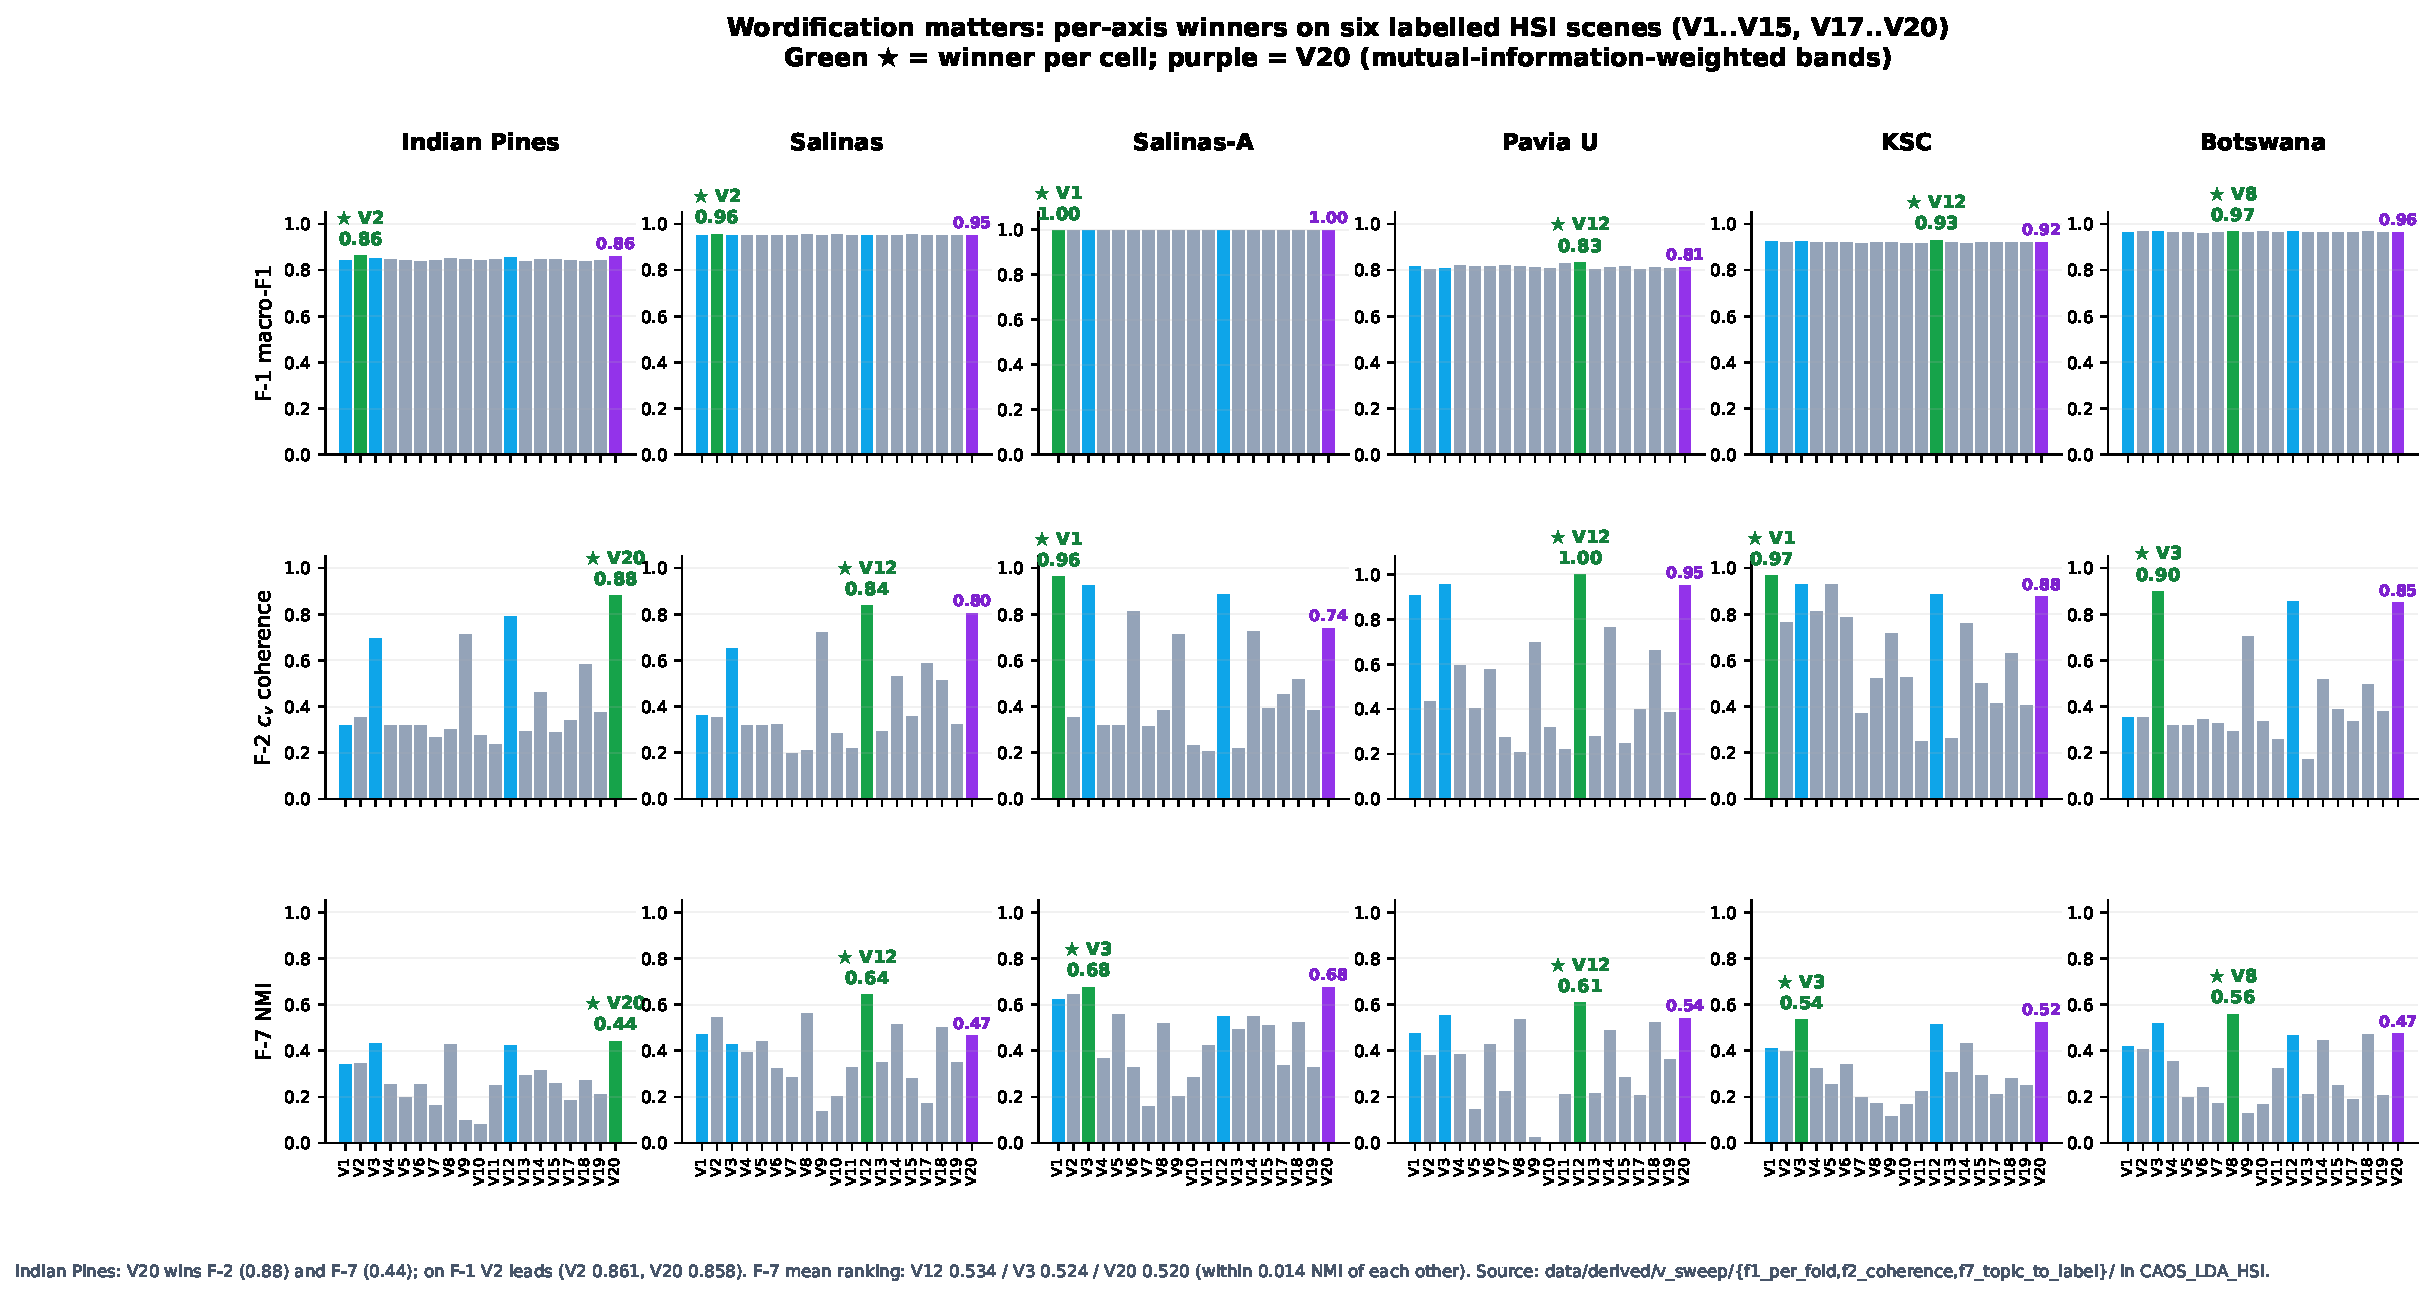
\includegraphics[width=\textwidth]{p3-winners-headline.pdf}
\caption{Headline. Per-axis winners on six labelled HSI scenes for
F-1 (5-fold macro-F1), F-2 ($c_v$ coherence) and F-7 (topic--label
NMI). Bars: green $\star$ = winner per cell; purple = V20 (MI-weighted
bands). Indian Pines (left column): V20 wins
F-2 and F-7 outright; on F-1 macro-F1 V2 leads (0.861, V20 0.858) and
the nineteen recipes span 0.837 to 0.861. F-7 mean ranking across the six scenes is V12 0.534 /
V3 0.524 / V20 0.520, within 0.014 NMI of each other at $Q=8$:
a flat top, not a sharp peak (the ranking inverts to a V20 lead at
$Q=32$).}
\label{fig:headline}
\end{figure*}

% =====================================================================
\section{Introduction}\label{sec:intro}
% =====================================================================

The companion paper~\cite{santibanezleal2026framework} (denoted P1
hereafter) proposes a twelve-axis
evaluation framework for LDA-style topic models on hyperspectral
imagery, instantiates it on a single \emph{canonical} wordification
recipe (V1, band--frequency tokens), and shows that classification
accuracy alone is silent about reproducibility, band robustness, and
calibration. P1's choice of V1 as canonical was a deliberate design
decision: every axis pulls a property of the same basis $\phi$, which
in turn requires that $\phi$ be fixed across axes. The decision was
defensible but it leaves an obvious second question unanswered:
\emph{does the choice of wordification itself change the conclusions?}

This paper answers that question. We define a family of nineteen
wordification recipes V1--V15 and V17--V20 that span the axes of design
freedom identified by the existing P1 code base
(\S\ref{sec:design-space}) and run each through the same evaluation
framework. The seven extension recipes V13--V15 and V17--V20 add
learnt-codebook tokens (V13 vector-quantised VAE, V17 sparse-coding
dictionary), signal-transform tokens (V14 continuous wavelet, V15
spectral indices), structure-aware tokens (V18 graph-Laplacian
eigenvectors, V19 UMAP coordinates) and a label-aware reweighting
(V20 mutual-information-weighted bands). The contribution is not a
new method but a comparative result: \emph{which recipe matters for
which axis on which scene}, and what that joint structure implies for
the choice of canonical recipe in future work. The V16 slot is
reserved for a foundation-model wordification (HyperSIGMA /
HyperspectralMAE), which is left to a follow-up study because its
inference cost would dominate the per-scene computational cost of the
labelled-scene panel.

\subsection{Why a sweep, not a winner}
\label{subsec:why-sweep}
A sweep is the right unit of analysis when no recipe is universally
better. The nineteen-recipe sweep on the six labelled scenes
shows that F-2 has four distinct winners (V1, V3, V12, V20), F-7 has
four distinct winners (V3, V8, V12, V20), and the three top recipes
across F-7 mean (V12, V3, V20) lie within $0.014$ NMI of each other.
V1 (current canonical) wins F-2 on two scenes and never wins F-7.
V20, the simplest label-aware reweighting of V3, wins both F-2
and F-7 on Indian Pines and is within 0.011 NMI of the F-7 leader on
two more scenes (Salinas-A and Kennedy SC).
Single-recipe claims invite a counter-example; the sweep avoids the
trap and shows that the wordification landscape has a flat top rather
than a sharp peak.

\subsection{Contributions}
\label{subsec:contributions}
\begin{enumerate}
  \item A formal definition of the V1--V15, V17--V20 wordification
    design space, spanning seven axes of freedom: token alphabet,
    spatial vs.\ purely spectral aggregation, local vs.\ global
    vocabulary, document length regime, signal transform, learnt vs.\
    fixed vocabulary, and label-aware vs.\ label-blind weighting
    (\S\ref{sec:design-space}).
  \item A per-recipe K-policy that keeps the comparison fair for
    extreme document-length regimes (V7 with $\le 6$ tokens per
    document, V9 with 1 token per document, V19 with 3 UMAP-axis
    tokens) where the canonical
    $K = \max(4, \min(12, n_{\text{classes}}))$ from P1 over-prescribes
    K (\S\ref{subsec:k-policy}).
  \item The nineteen-recipe result matrix on the six labelled scenes
    of the P1 panel for F-1, F-2 and F-7, with unpaired bootstrap
    intervals on F-1 macro-F1 for V1--V12 and paired (scene, fold)
    comparisons for all nineteen recipes
    (\S\ref{sec:results}--\ref{sec:matrix}).
  \item Four \emph{axis--recipe affinities} observed in the sweep:
    V3 vs.\ F-7 (three scene wins in the twelve-recipe view, one of them
    by 0.002; ahead of V1 on four of five scenes), V12 vs.\ F-2 on dense regimes, V20 vs.\ F-7
    NMI on label-information-bearing scenes, and V18 vs.\ F-7 on
    manifold-shaped scenes (Pavia~U, Salinas) among the unsupervised
    structure-aware extension recipes; a fifth, V7 vs.\ F-9 on HIDSAG, is stated
    as a hypothesis that this study does not test
    (\S\ref{sec:affinities}).
  \item A revised recommendation for the role of V1 going forward:
    \emph{a reproducibility default, not a universal best}
    (\S\ref{sec:recommendation}).
\end{enumerate}

\subsection{Paper organisation}
\S\ref{sec:design-space} formalises the nineteen recipes.
\S\ref{sec:method} states the per-recipe K-policy and the rest of the
experimental setup (carried over verbatim from P1 except where noted).
\S\ref{sec:results} reports F-1 (classification),
\S\ref{sec:f2-results} F-2 (coherence), \S\ref{sec:f7-results} F-7
(topic--label coupling). \S\ref{sec:f-extension-results} narrows
F-2 and F-7 to the V13--V20 extension and discusses each extension
recipe mechanistically. \S\ref{sec:matrix} stitches the per-axis
results into the joint matrix. \S\ref{sec:affinities} discusses the
four observed axis--recipe affinities and one hypothesis; \S\ref{sec:recommendation}
makes the canonical-default recommendation; \S\ref{sec:limitations}
notes limitations (the nanopq seeding issue on V11; the
sliding-window estimator gap for $c_{\mathrm{NPMI}}$ on dense recipes; the
deferred F-3 / F-4 / F-5 / F-8 / F-9 / F-10 / F-11 / F-12 sweeps; the
V16 foundation-model wordification deferred to a follow-up).
Appendix~\ref{app:full-matrix} reproduces the full 19-recipe matrices.

% =====================================================================
\section{Related work}\label{sec:related}
% =====================================================================

\paragraph{Topic models} Latent Dirichlet allocation
\cite{blei2003lda} and its collapsed-Gibbs \cite{griffiths2004finding}
and online-variational \cite{hoffman2010online} estimators are the
backbone this paper sweeps over; we use the online-VB implementation
\eqref{eq:lda-gen}. The nonparametric hierarchical Dirichlet process
\cite{teh2006hdp} \eqref{eq:hdp-gen} and the neural topic models
ProdLDA \cite{srivastava2017autoencoding} \eqref{eq:prodlda-gen} and
the embedded topic model \cite{dieng2020topic} \eqref{eq:etm-beta}
(the latter built on neural variational inference \cite{miao2016neural}
and the variational autoencoder \cite{kingma2014auto}) enter as the
alternative backbones of the cross-backbone factorial
(\S\ref{sec:extensions}). The model run under the ProdLDA label is the
mixture-decoder form of Srivastava and Sutton's amortised topic model
(their NVLDA): a standard normal prior $\delta_d \sim \mathcal{N}(0, I)$,
$\theta_d = \mathrm{softmax}(\delta_d)$ and
$w_{dn} \sim \mathrm{Cat}(\sum_k \theta_{dk} \beta_k)$ with
$\beta_k = \mathrm{softmax}(\omega_k)$ from free topic--word logits
$\omega_k$; the product-of-experts decoder that
defines ProdLDA was not run. ETM has the same prior and amortised encoder
and the decoder $\beta_k = \mathrm{softmax}(\rho^{\top}\alpha_k)$ with word
embeddings of dimension $L = 64$ and a mixture likelihood, so the two
neural backbones differ only in the decoder parameterisation (a free
$K \times |V|$ topic--word matrix against a rank-$L$ factorisation).
Model selection over $K$ is informed by the
estimation-and-selection analysis of \cite{taddy2012estimation}.

\paragraph{LDA and topic models on hyperspectral and spectral data}
Probabilistic topic models have been applied to spectral data for
subpixel unmixing \cite{zou2017pmlda}, plant-phenotyping spectroscopy
\cite{wahabzada2015plant}, and geometallurgical estimation from
hyperspectral core imagery \cite{santibanezleal2022procemin}, which
introduced the band--frequency document recipes that V1--V3 generalise
here. The broader hyperspectral classification and unmixing literature
\cite{plaza2009recent,camps2014advances,bioucasdias2012unmixing}
supplies the endmember-extraction machinery behind V8: NFINDR-style
simplex-vertex endmembers, with vertex component analysis
\cite{nascimento2005vca} as the closely-related fast alternative and
\cite{borsoi2021variability} surveying spectral-variability effects on
the abundances V8 quantises.

\paragraph{Coherence, reliability, and evaluation} F-2 uses the $c_v$
coherence of \cite{roder2015exploring} \eqref{eq:f2}, which generalises
the human-judgement-correlated PMI/NPMI measures of
\cite{newman2010coherence} and the document-co-occurrence statistic of
\cite{mimno2011coherence}. F-7 reports a mutual information normalised by the label entropy $H(Y)$
\eqref{eq:f7}, i.e.\ the asymmetric uncertainty coefficient $U(Y\mid\hat
Z)=I(\hat Z;Y)/H(Y)$ (not chance-corrected); the normalisation follows the
conventions catalogued by \cite{vinh2010information}. Because the topic
count $K$ varies across recipes and backbones, this uncorrected score
carries a mild $K$-dependent upward bias and is best read within, rather
than strictly across, recipes of differing $K$. F-18 instantiates the multi-seed
stability protocol of \cite{greene2014topics} using Hungarian matching
\cite{kuhn1955hungarian,munkres1957algorithms} of top-$N$ indicator
sets \eqref{eq:f18}. The uniform-quantiser distortion bound of
\cite{gershogray1992vq} bounds the wordification noise introduced by
the $Q$-level binning in \eqref{eq:quantiser}. We follow the
reproducibility recommendations of \cite{pineau2021nature} and build on
the scikit-learn \cite{pedregosa2011scikit}, NumPy
\cite{harris2020numpy}, SciPy \cite{virtanen2020scipy} and gensim
\cite{rehurek2010gensim} implementations; the mutual-information
weighting in V20 \eqref{eq:v20} uses the \texttt{mutual\_info\_classif}
estimator of \cite{pedregosa2011scikit}.

% =====================================================================
\section{The nineteen-recipe wordification design space}
\label{sec:design-space}
% =====================================================================

\begin{figure*}[t]
\centering
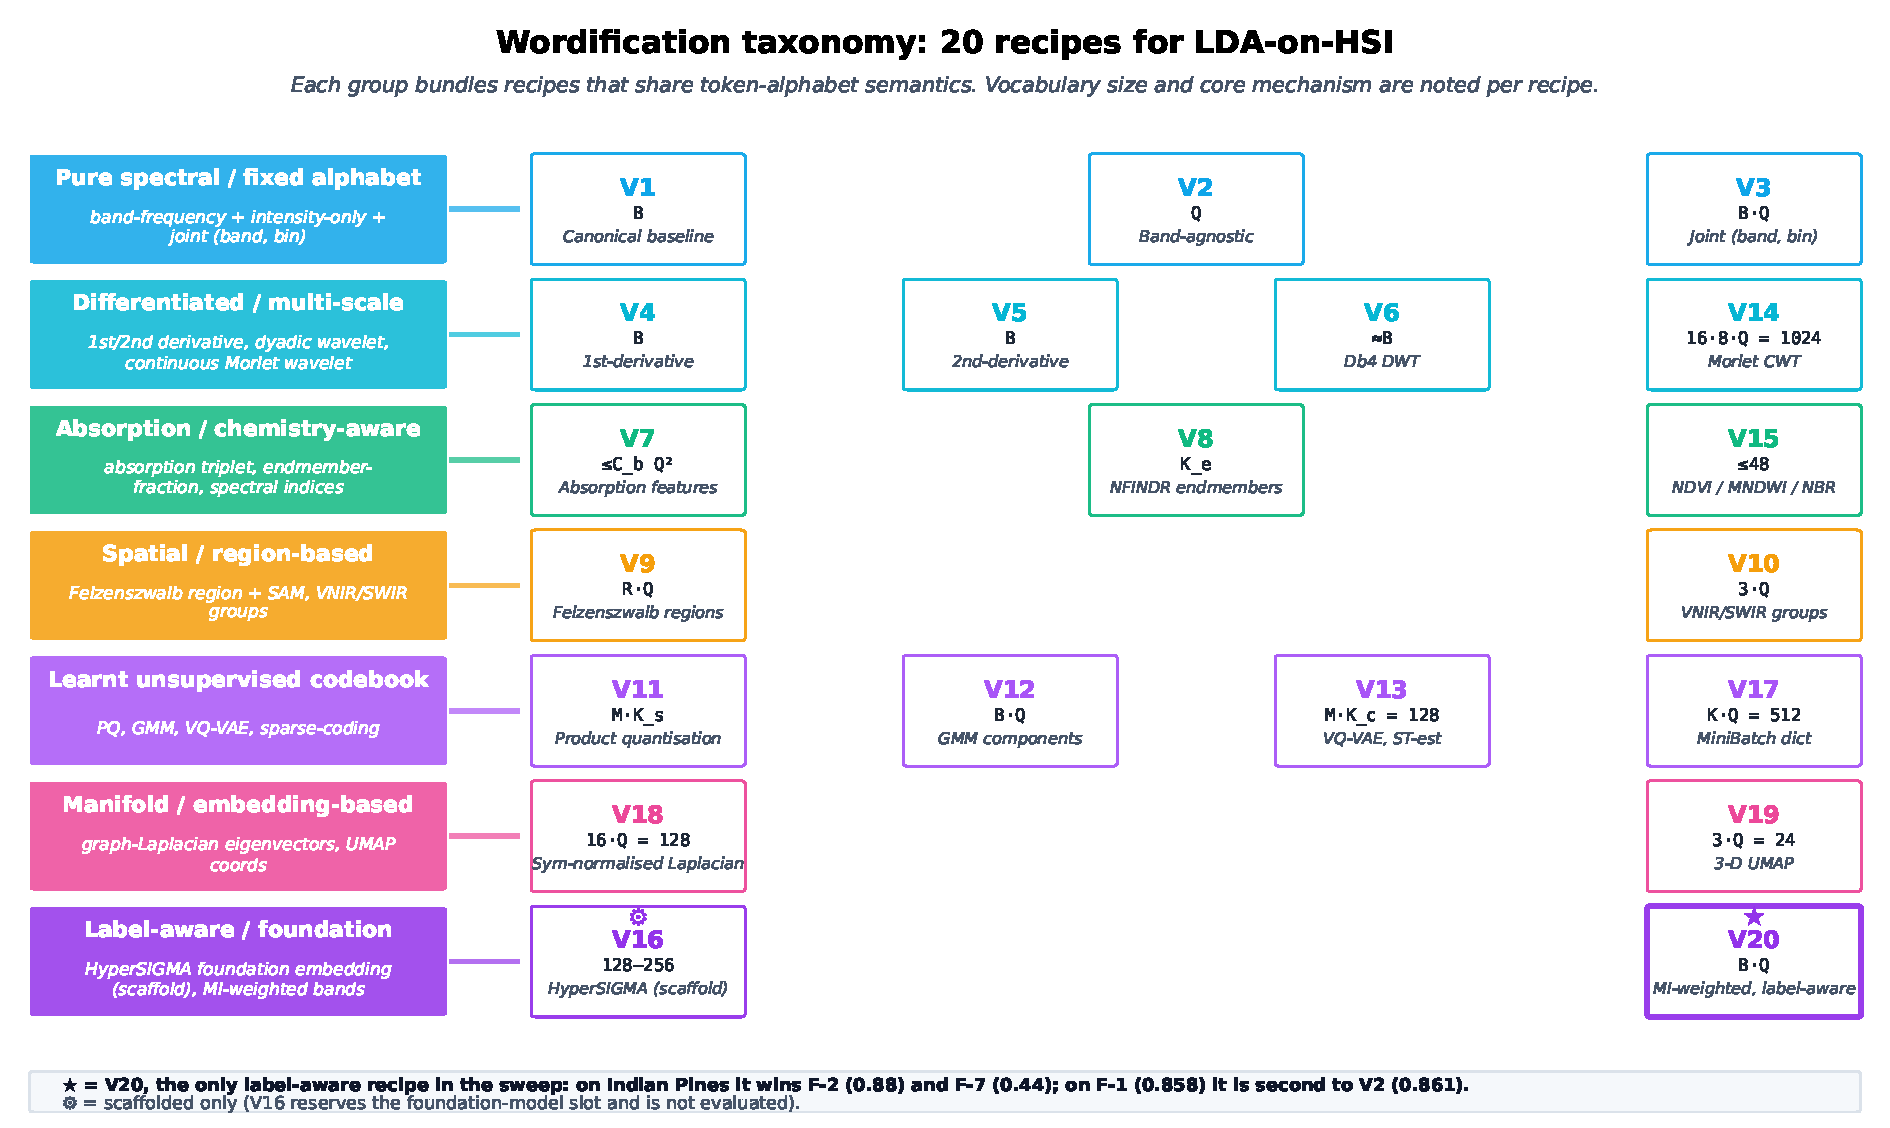
\includegraphics[width=0.95\textwidth]{wordification-taxonomy.pdf}
\caption{The wordification taxonomy. Twenty recipes are grouped into
seven families by token-alphabet semantics. V20 (purple, $\star$) is the
only label-aware recipe in the sweep; it wins F-2 and F-7 together on
Indian Pines, where it is second to V2 on F-1 (0.858 against 0.861). V16
(HyperSIGMA foundation-model embedding) is scaffolded only and is not
evaluated: its pretrained weights are not integrated.}
\label{fig:taxonomy}
\end{figure*}

% ---------------------------------------------------------------------
% Canonical equation set, shared across the P3/P4/P5 manuscript series.
% Single source of truth: ../../equations/canonical.tex. We \input it
% here and reference the labels by \eqref{} throughout; the displayed
% equations therefore stay byte-identical across all papers in the
% series. The LDA backbone \eqref{eq:lda-gen}, the quantiser
% \eqref{eq:quantiser}, the five reference recipes
% \eqref{eq:v1}/\eqref{eq:v3}/\eqref{eq:v8}/\eqref{eq:v12}/\eqref{eq:v20},
% and the six evaluation axes \eqref{eq:f1}--\eqref{eq:f22} are all
% defined there. Unused groups (HDP/ProdLDA/ETM backbones, F-15,
% dispersion, affinity) are also typeset for cross-paper coherence.
% ---------------------------------------------------------------------
% ===================================================================
% CANONICAL EQUATION SET: CAOS_LDA_HSI manuscript series (P3/P4/P5)
% ===================================================================
% Single source of truth for all display equations. Authored once,
% \input into P3 (journal_v_sweep), P4 (journal_backbone_factorial),
% P5 (journal_interpretability), and transcribed (KaTeX) into the
% web-app methodology route and the wiki Mathematical-Background page.
%
% Usage:  % ===================================================================
% CANONICAL EQUATION SET: CAOS_LDA_HSI manuscript series (P3/P4/P5)
% ===================================================================
% Single source of truth for all display equations. Authored once,
% \input into P3 (journal_v_sweep), P4 (journal_backbone_factorial),
% P5 (journal_interpretability), and transcribed (KaTeX) into the
% web-app methodology route and the wiki Mathematical-Background page.
%
% Usage:  % ===================================================================
% CANONICAL EQUATION SET: CAOS_LDA_HSI manuscript series (P3/P4/P5)
% ===================================================================
% Single source of truth for all display equations. Authored once,
% \input into P3 (journal_v_sweep), P4 (journal_backbone_factorial),
% P5 (journal_interpretability), and transcribed (KaTeX) into the
% web-app methodology route and the wiki Mathematical-Background page.
%
% Usage:  \input{../../equations/canonical.tex}  then reference the
% groups by \eqref{eq:lda-gen}, \eqref{eq:etm-beta}, etc. Groups can
% also be copied verbatim into a single \begin{align} if a paper wants
% them inline. Each equation is independently labelled.
%
% NOTATION (fixed once, used everywhere):
%   b in {1..B}    spectral band            (B ~ 200)
%   q in {0..Q-1}  quantisation level       (Q in {8,16,32}, default 8)
%   k in {1..K}    topic                    (K per-scene K-policy)
%   d in {1..D}    document = labelled pixel
%   v in V         wordification vocabulary (recipe-specific)
%   x_d in R^B     normalised pixel spectrum
%   y_d            land-cover / mineral label of pixel d
%   theta_d        per-doc topic proportions  (simplex Delta^{K-1})
%   phi_k          topic-word distribution    (simplex Delta^{|V|-1})
%   n_d in N^{|V|} doc-term count vector produced by a recipe
% ===================================================================

% ----- GROUP A : the four topic-model backbones -------------------

% A1  LDA (online variational Bayes; P1/P3 baseline)
\begin{equation}\label{eq:lda-gen}
\begin{gathered}
\phi_k \sim \mathrm{Dir}(\beta),\quad
\theta_d \sim \mathrm{Dir}(\alpha),\\
z_{dn} \sim \mathrm{Cat}(\theta_d),\quad
w_{dn} \sim \mathrm{Cat}(\phi_{z_{dn}}).
\end{gathered}
\end{equation}

% A2  HDP (nonparametric K via two-level stick-breaking)
\begin{equation}\label{eq:hdp-gen}
\begin{gathered}
\boldsymbol{\beta}\sim\mathrm{GEM}(\gamma),\quad
\pi_d \sim \mathrm{DP}(\alpha_0,\boldsymbol{\beta}),\\
z_{dn}\sim\mathrm{Cat}(\pi_d),\quad
w_{dn}\sim\mathrm{Cat}(\phi_{z_{dn}}),
\end{gathered}
\end{equation}
with global atom weights $\beta_k=\beta'_k\prod_{l<k}(1-\beta'_l)$,
$\beta'_k\sim\mathrm{Beta}(1,\gamma)$.

% A3  "ProdLDA" as run: the amortised neural topic model of Srivastava and Sutton
%     in its mixture-decoder form (their NVLDA), with a standard normal prior on
%     the topic-proportion logits delta_d and a free matrix of unnormalised
%     topic-word logits omega_k (no product of experts, no Laplace approximation)
\begin{equation}\label{eq:prodlda-gen}
\begin{gathered}
\delta_d \sim \mathcal{N}(0, I),\quad
\theta_d = \mathrm{softmax}(\delta_d),\\
\beta_k = \mathrm{softmax}(\omega_k),\quad
w_{dn} \sim \mathrm{Cat}\!\Big(\textstyle\sum_k \theta_{dk}\,\beta_k\Big),
\end{gathered}
\end{equation}
where the unnormalised topic--word logits $\omega_k\in\mathbb{R}^{|V|}$ form
a free $K\times|V|$ matrix and inference is amortised,
$(\mu_d,\Sigma_d)=\mathrm{Enc}_\eta(n_d)$. ProdLDA as published mixes the
logits instead, $w_{dn}\sim\mathrm{Cat}\big(\mathrm{softmax}(\textstyle\sum_k \theta_{dk}\,\omega_k)\big)$
(a product of experts), with a Laplace approximation to $\mathrm{Dir}(\alpha)$
as the prior; that form was not run.

% A4  ETM (embedded topic model; same prior and encoder as A3, rank-L decoder)
\begin{equation}\label{eq:etm-beta}
\begin{gathered}
\delta_d \sim \mathcal{N}(0, I),\quad
\theta_d = \mathrm{softmax}(\delta_d),\\
\beta_k = \mathrm{softmax}\!\big(\rho^{\top}\alpha_k\big),\quad
w_{dn}\sim\mathrm{Cat}\!\Big(\textstyle\sum_k \theta_{dk}\,\beta_k\Big),
\end{gathered}
\end{equation}
with word embeddings $\rho\in\mathbb{R}^{L\times|V|}$ and topic
embeddings $\alpha_k\in\mathbb{R}^{L}$ ($L=64$), and the same amortised
encoder as \eqref{eq:prodlda-gen}.

% ----- GROUP B : wordification recipes (spectrum -> doc-term) ------

% B0  per-row min-max normalisation + uniform quantiser
\begin{equation}\label{eq:quantiser}
\begin{gathered}
\tilde{x}_{db}=\frac{x_{db}-\min_b x_{db}}{\max_b x_{db}-\min_b x_{db}},
\\
q_b(x_d)=\mathrm{clip}\big(\lfloor \tilde{x}_{db}\,Q\rfloor,\,0,\,Q-1\big).
\end{gathered}
\end{equation}

% B1  V1 band-frequency: token = band, multiplicity = quantised intensity
\begin{equation}\label{eq:v1}
n_d^{\mathrm{V1}}[b] = q_b(x_d),\qquad |V_{\mathrm{V1}}| = B.
\end{equation}

% B2  V3 joint (band, bin): one token per band naming its bin
\begin{equation}\label{eq:v3}
n_d^{\mathrm{V3}}[(b,q)] = \mathds{1}\!\left[q_b(x_d)=q\right],\qquad
|V_{\mathrm{V3}}| = B\,Q .
\end{equation}

% B3  V8 NFINDR endmember-fraction: FCLS abundances, rescaled by the pixel's largest abundance and
%     quantised to Q levels (build_wordifications_v6plus.wordify_v8_endmember_fraction)
\begin{equation}\label{eq:v8}
\begin{gathered}
a_d=\arg\min_{a\ge 0,\;\mathbf{1}^{\top}a=1}\;\lVert x_d - E\,a\rVert_2^2,\\
n_d^{\mathrm{V8}}[m]=\min\!\Big(\Big\lfloor Q\,\frac{a_{dm}}{\max_{m'} a_{dm'}}\Big\rfloor,\;Q-1\Big),
\end{gathered}
\end{equation}
where $E=[e_1,\dots,e_M]$ are the NFINDR endmembers (simplex vertices),
$x_d$ is the unnormalised spectrum and $|V_{\mathrm{V8}}|=M$. The abundance
non-negativity (ANC, $a\ge 0$) and sum-to-one (ASC, $\mathbf{1}^{\top}a=1$)
constraints make $a_d$ a point on the simplex spanned by the endmembers
(fully-constrained least squares, FCLS; implemented as
$\delta$-augmented NNLS followed by renormalisation), so the coefficients
are proper abundance fractions over the convex hull. The dominant
endmember of every pixel emits $Q-1$ tokens, so the document length
grows with $Q$.

% B4  V12 GMM-token: (band, component) joints from one 1-D Q-component Gaussian mixture fitted to the
%     band intensities (build_wordifications_v6plus.wordify_v12_gmm; hard assignment, not responsibilities)
\begin{equation}\label{eq:v12}
\begin{gathered}
g_b(x_d)=\arg\max_{k\in\{0,\dots,Q-1\}}\;\pi_k\,\mathcal{N}\big(x_{db}\mid\mu_k,\sigma_k^2\big),\\
n_d^{\mathrm{V12}}[(b,g)]=\mathds{1}\!\left[g_b(x_d)=g\right],\qquad
|V_{\mathrm{V12}}|=B\,Q,
\end{gathered}
\end{equation}
where $(\pi_k,\mu_k,\sigma_k^2)_{k<Q}$ is a one-dimensional Gaussian
mixture fitted once per scene to the unnormalised band intensities of the
sampled pixels (a random subset of 50\,000 values), with the components
indexed in increasing order of $\mu_k$. Each band emits one token, as in
V3, but the bins are shared by all pixels and follow the intensity
distribution instead of splitting each spectrum's own range into equal
intervals.

% B5  V20 MI-weighted bands: V3 alphabet, per-band emission multiplicity
\begin{equation}\label{eq:v20}
\begin{gathered}
w_b=\Big\lfloor \tfrac{\mathrm{MI}(x_{\cdot b};\,y)}{\max_{b'}\mathrm{MI}(x_{\cdot b'};\,y)}\;Q_{\max}\Big\rceil,
\\
n_d^{\mathrm{V20}}[(b,q)] = w_b\,\mathds{1}\!\left[q_b(x_d)=q\right].
\end{gathered}
\end{equation}
The token alphabet is V3's, $|V_{\mathrm{V20}}|=B\,Q$ (=1600 at
$B=200,Q=8$; mean $\approx 1376$ across the six labelled scenes since
$B$ varies). Bands with $w_b=0$ emit nothing, so the \emph{effective}
(non-empty-column) vocabulary is smaller still ($\approx 770$ mean).

% ----- GROUP C : evaluation axes ----------------------------------

% C1  F-1 macro-F1 (5-fold; topic_routed_soft head)
\begin{equation}\label{eq:f1}
\mathrm{F\text{-}1}=\frac{1}{|\mathcal{C}|}\sum_{c\in\mathcal{C}}
\frac{2\,P_c R_c}{P_c+R_c}.
\end{equation}

% C2  F-2 coherence c_v (NPMI sliding window + cosine aggregation)
\begin{equation}\label{eq:f2}
\begin{gathered}
\mathrm{NPMI}(w_i,w_j)=\frac{\log\frac{p(w_i,w_j)+\epsilon}{p(w_i)p(w_j)}}{-\log\big(p(w_i,w_j)+\epsilon\big)},\\
c_v=\frac{1}{N}\sum_{i}\cos\!\big(\mathbf{v}_i,\,\textstyle\sum_j \mathbf{v}_j\big),
\end{gathered}
\end{equation}
with $\mathbf{v}_i=\big(\mathrm{NPMI}(w_i,w_\ell)\big)_{\ell=1}^{N}$ over the
top-$N$ topic words.

% C3  F-7 topic-to-label MI normalised by H(label) -- this is the
% ASYMMETRIC label-normalised MI (uncertainty coefficient U(Y|Zhat) =
% completeness, Rosenberg-Hirschberg 2007), NOT the symmetric NMI
% I/sqrt(H H). Uncorrected for chance.
\begin{equation}\label{eq:f7}
\begin{gathered}
\hat{z}_d=\arg\max_k \theta_{dk},\\
\mathrm{F\text{-}7}=\frac{I(\hat{Z};Y)}{H(Y)}
\;=\; U(Y\mid\hat{Z})\;=\;1-\frac{H(Y\mid\hat{Z})}{H(Y)}.
\end{gathered}
\end{equation}

% C4  F-14 top-N pairwise Jaccard repetitiveness (lower = more diverse)
\begin{equation}\label{eq:f14}
\mathrm{F\text{-}14}=\frac{2}{K(K-1)}\sum_{k<k'}
\frac{|T_k\cap T_{k'}|}{|T_k\cup T_{k'}|},\qquad T_k=\text{top-}N(\phi_k).
\end{equation}

% C5  F-18 Maier reseed reliability (Hungarian-matched top-N cosine)
\begin{equation}\label{eq:f18}
\mathrm{F\text{-}18}=\frac{1}{\binom{S}{2}}\sum_{s<s'}\frac{1}{K}
\max_{\sigma\in\mathfrak{S}_K}\sum_{k}\cos\!\big(\mathbf{u}^{(s)}_k,\mathbf{u}^{(s')}_{\sigma(k)}\big),
\end{equation}
over $S$ reseeded refits, with $\mathbf{u}^{(s)}_k$ the top-$N$ indicator
vector of topic $k$ in run $s$.

% C6  F-22 counterfactual L1 (min token perturbation to flip argmax topic)
\begin{equation}\label{eq:f22}
\begin{aligned}
\mathrm{F\text{-}22}(d)={}&\min_{\delta\in\mathbb{Z}^{|V|}}\lVert\delta\rVert_1
\;\;\text{s.t.}\\
&\arg\max_k\theta_k(n_d+\delta)\neq\arg\max_k\theta_k(n_d),\\
&n_d+\delta\ge 0,
\end{aligned}
\end{equation}
reported as the per-scene median, capped at a sentinel
$\mathrm{MAX\_STEPS}=50$ when no flip is found.

% C7  F-15 LLM-judge alignment (top-N overlap rule, as the judge implementation computes it:
%     ambiguous documents, i.e. neither aligned nor with >= 3 non-zero tokens, are excluded)
\begin{equation}\label{eq:f15}
\begin{aligned}
\mathrm{aligned}(d)&=\mathds{1}\big[\,|\mathrm{top}_N(n_d)\cap\mathrm{top}_N(\phi_{\hat{z}_d})|\ge\tau\\
&\qquad\;\vee\;\mathrm{top}_3(n_d)\cap\mathrm{top}_N(\phi_{\hat{z}_d})\neq\emptyset\,\big],\\
\mathrm{decisive}(d)&=\mathds{1}\big[\,\mathrm{aligned}(d)=1\;\vee\;|\mathrm{supp}(n_d)|\ge 3\,\big],\\
\mathrm{F\text{-}15}&=\textstyle\sum_d \mathrm{aligned}(d)\,\big/\textstyle\sum_d \mathrm{decisive}(d).
\end{aligned}
\end{equation}

% C8  token-mass dispersion (P5 mechanism metric: effective vocabulary)
\begin{equation}\label{eq:dispersion}
\begin{gathered}
p_{dv}=\frac{n_{dv}}{\sum_{v'} n_{dv'}},\\
N_{\mathrm{eff}}(d)=\exp\!\big(H(p_d)\big)=\exp\!\Big(-\sum_v p_{dv}\log p_{dv}\Big).
\end{gathered}
\end{equation}
$N_{\mathrm{eff}}$ counts the tokens that effectively carry the mass of
$p_d$ (or of a topic's $\phi_k$): it is low when the mass is concentrated
on few tokens and at most $|V|$.

% ----- GROUP D : cross-backbone affinity score (P4) ----------------

% D1  per-recipe cross-backbone affinity (min-max normalised within backbone)
\begin{equation}\label{eq:affinity}
\mathcal{A}(V_i)=\frac{1}{|\mathcal{B}|}\sum_{m\in\mathcal{B}}
\frac{c_v^{(m)}(V_i)-\min_j c_v^{(m)}(V_j)}{\max_j c_v^{(m)}(V_j)-\min_j c_v^{(m)}(V_j)}\;\in[0,1],
\end{equation}
averaged over backbones $\mathcal{B}=\{\mathrm{LDA},\mathrm{HDP},\mathrm{ProdLDA},\mathrm{ETM}\}$;
$\mathcal{A}\to 1$ when a recipe sits near the per-backbone top everywhere.
  then reference the
% groups by \eqref{eq:lda-gen}, \eqref{eq:etm-beta}, etc. Groups can
% also be copied verbatim into a single \begin{align} if a paper wants
% them inline. Each equation is independently labelled.
%
% NOTATION (fixed once, used everywhere):
%   b in {1..B}    spectral band            (B ~ 200)
%   q in {0..Q-1}  quantisation level       (Q in {8,16,32}, default 8)
%   k in {1..K}    topic                    (K per-scene K-policy)
%   d in {1..D}    document = labelled pixel
%   v in V         wordification vocabulary (recipe-specific)
%   x_d in R^B     normalised pixel spectrum
%   y_d            land-cover / mineral label of pixel d
%   theta_d        per-doc topic proportions  (simplex Delta^{K-1})
%   phi_k          topic-word distribution    (simplex Delta^{|V|-1})
%   n_d in N^{|V|} doc-term count vector produced by a recipe
% ===================================================================

% ----- GROUP A : the four topic-model backbones -------------------

% A1  LDA (online variational Bayes; P1/P3 baseline)
\begin{equation}\label{eq:lda-gen}
\begin{gathered}
\phi_k \sim \mathrm{Dir}(\beta),\quad
\theta_d \sim \mathrm{Dir}(\alpha),\\
z_{dn} \sim \mathrm{Cat}(\theta_d),\quad
w_{dn} \sim \mathrm{Cat}(\phi_{z_{dn}}).
\end{gathered}
\end{equation}

% A2  HDP (nonparametric K via two-level stick-breaking)
\begin{equation}\label{eq:hdp-gen}
\begin{gathered}
\boldsymbol{\beta}\sim\mathrm{GEM}(\gamma),\quad
\pi_d \sim \mathrm{DP}(\alpha_0,\boldsymbol{\beta}),\\
z_{dn}\sim\mathrm{Cat}(\pi_d),\quad
w_{dn}\sim\mathrm{Cat}(\phi_{z_{dn}}),
\end{gathered}
\end{equation}
with global atom weights $\beta_k=\beta'_k\prod_{l<k}(1-\beta'_l)$,
$\beta'_k\sim\mathrm{Beta}(1,\gamma)$.

% A3  "ProdLDA" as run: the amortised neural topic model of Srivastava and Sutton
%     in its mixture-decoder form (their NVLDA), with a standard normal prior on
%     the topic-proportion logits delta_d and a free matrix of unnormalised
%     topic-word logits omega_k (no product of experts, no Laplace approximation)
\begin{equation}\label{eq:prodlda-gen}
\begin{gathered}
\delta_d \sim \mathcal{N}(0, I),\quad
\theta_d = \mathrm{softmax}(\delta_d),\\
\beta_k = \mathrm{softmax}(\omega_k),\quad
w_{dn} \sim \mathrm{Cat}\!\Big(\textstyle\sum_k \theta_{dk}\,\beta_k\Big),
\end{gathered}
\end{equation}
where the unnormalised topic--word logits $\omega_k\in\mathbb{R}^{|V|}$ form
a free $K\times|V|$ matrix and inference is amortised,
$(\mu_d,\Sigma_d)=\mathrm{Enc}_\eta(n_d)$. ProdLDA as published mixes the
logits instead, $w_{dn}\sim\mathrm{Cat}\big(\mathrm{softmax}(\textstyle\sum_k \theta_{dk}\,\omega_k)\big)$
(a product of experts), with a Laplace approximation to $\mathrm{Dir}(\alpha)$
as the prior; that form was not run.

% A4  ETM (embedded topic model; same prior and encoder as A3, rank-L decoder)
\begin{equation}\label{eq:etm-beta}
\begin{gathered}
\delta_d \sim \mathcal{N}(0, I),\quad
\theta_d = \mathrm{softmax}(\delta_d),\\
\beta_k = \mathrm{softmax}\!\big(\rho^{\top}\alpha_k\big),\quad
w_{dn}\sim\mathrm{Cat}\!\Big(\textstyle\sum_k \theta_{dk}\,\beta_k\Big),
\end{gathered}
\end{equation}
with word embeddings $\rho\in\mathbb{R}^{L\times|V|}$ and topic
embeddings $\alpha_k\in\mathbb{R}^{L}$ ($L=64$), and the same amortised
encoder as \eqref{eq:prodlda-gen}.

% ----- GROUP B : wordification recipes (spectrum -> doc-term) ------

% B0  per-row min-max normalisation + uniform quantiser
\begin{equation}\label{eq:quantiser}
\begin{gathered}
\tilde{x}_{db}=\frac{x_{db}-\min_b x_{db}}{\max_b x_{db}-\min_b x_{db}},
\\
q_b(x_d)=\mathrm{clip}\big(\lfloor \tilde{x}_{db}\,Q\rfloor,\,0,\,Q-1\big).
\end{gathered}
\end{equation}

% B1  V1 band-frequency: token = band, multiplicity = quantised intensity
\begin{equation}\label{eq:v1}
n_d^{\mathrm{V1}}[b] = q_b(x_d),\qquad |V_{\mathrm{V1}}| = B.
\end{equation}

% B2  V3 joint (band, bin): one token per band naming its bin
\begin{equation}\label{eq:v3}
n_d^{\mathrm{V3}}[(b,q)] = \mathds{1}\!\left[q_b(x_d)=q\right],\qquad
|V_{\mathrm{V3}}| = B\,Q .
\end{equation}

% B3  V8 NFINDR endmember-fraction: FCLS abundances, rescaled by the pixel's largest abundance and
%     quantised to Q levels (build_wordifications_v6plus.wordify_v8_endmember_fraction)
\begin{equation}\label{eq:v8}
\begin{gathered}
a_d=\arg\min_{a\ge 0,\;\mathbf{1}^{\top}a=1}\;\lVert x_d - E\,a\rVert_2^2,\\
n_d^{\mathrm{V8}}[m]=\min\!\Big(\Big\lfloor Q\,\frac{a_{dm}}{\max_{m'} a_{dm'}}\Big\rfloor,\;Q-1\Big),
\end{gathered}
\end{equation}
where $E=[e_1,\dots,e_M]$ are the NFINDR endmembers (simplex vertices),
$x_d$ is the unnormalised spectrum and $|V_{\mathrm{V8}}|=M$. The abundance
non-negativity (ANC, $a\ge 0$) and sum-to-one (ASC, $\mathbf{1}^{\top}a=1$)
constraints make $a_d$ a point on the simplex spanned by the endmembers
(fully-constrained least squares, FCLS; implemented as
$\delta$-augmented NNLS followed by renormalisation), so the coefficients
are proper abundance fractions over the convex hull. The dominant
endmember of every pixel emits $Q-1$ tokens, so the document length
grows with $Q$.

% B4  V12 GMM-token: (band, component) joints from one 1-D Q-component Gaussian mixture fitted to the
%     band intensities (build_wordifications_v6plus.wordify_v12_gmm; hard assignment, not responsibilities)
\begin{equation}\label{eq:v12}
\begin{gathered}
g_b(x_d)=\arg\max_{k\in\{0,\dots,Q-1\}}\;\pi_k\,\mathcal{N}\big(x_{db}\mid\mu_k,\sigma_k^2\big),\\
n_d^{\mathrm{V12}}[(b,g)]=\mathds{1}\!\left[g_b(x_d)=g\right],\qquad
|V_{\mathrm{V12}}|=B\,Q,
\end{gathered}
\end{equation}
where $(\pi_k,\mu_k,\sigma_k^2)_{k<Q}$ is a one-dimensional Gaussian
mixture fitted once per scene to the unnormalised band intensities of the
sampled pixels (a random subset of 50\,000 values), with the components
indexed in increasing order of $\mu_k$. Each band emits one token, as in
V3, but the bins are shared by all pixels and follow the intensity
distribution instead of splitting each spectrum's own range into equal
intervals.

% B5  V20 MI-weighted bands: V3 alphabet, per-band emission multiplicity
\begin{equation}\label{eq:v20}
\begin{gathered}
w_b=\Big\lfloor \tfrac{\mathrm{MI}(x_{\cdot b};\,y)}{\max_{b'}\mathrm{MI}(x_{\cdot b'};\,y)}\;Q_{\max}\Big\rceil,
\\
n_d^{\mathrm{V20}}[(b,q)] = w_b\,\mathds{1}\!\left[q_b(x_d)=q\right].
\end{gathered}
\end{equation}
The token alphabet is V3's, $|V_{\mathrm{V20}}|=B\,Q$ (=1600 at
$B=200,Q=8$; mean $\approx 1376$ across the six labelled scenes since
$B$ varies). Bands with $w_b=0$ emit nothing, so the \emph{effective}
(non-empty-column) vocabulary is smaller still ($\approx 770$ mean).

% ----- GROUP C : evaluation axes ----------------------------------

% C1  F-1 macro-F1 (5-fold; topic_routed_soft head)
\begin{equation}\label{eq:f1}
\mathrm{F\text{-}1}=\frac{1}{|\mathcal{C}|}\sum_{c\in\mathcal{C}}
\frac{2\,P_c R_c}{P_c+R_c}.
\end{equation}

% C2  F-2 coherence c_v (NPMI sliding window + cosine aggregation)
\begin{equation}\label{eq:f2}
\begin{gathered}
\mathrm{NPMI}(w_i,w_j)=\frac{\log\frac{p(w_i,w_j)+\epsilon}{p(w_i)p(w_j)}}{-\log\big(p(w_i,w_j)+\epsilon\big)},\\
c_v=\frac{1}{N}\sum_{i}\cos\!\big(\mathbf{v}_i,\,\textstyle\sum_j \mathbf{v}_j\big),
\end{gathered}
\end{equation}
with $\mathbf{v}_i=\big(\mathrm{NPMI}(w_i,w_\ell)\big)_{\ell=1}^{N}$ over the
top-$N$ topic words.

% C3  F-7 topic-to-label MI normalised by H(label) -- this is the
% ASYMMETRIC label-normalised MI (uncertainty coefficient U(Y|Zhat) =
% completeness, Rosenberg-Hirschberg 2007), NOT the symmetric NMI
% I/sqrt(H H). Uncorrected for chance.
\begin{equation}\label{eq:f7}
\begin{gathered}
\hat{z}_d=\arg\max_k \theta_{dk},\\
\mathrm{F\text{-}7}=\frac{I(\hat{Z};Y)}{H(Y)}
\;=\; U(Y\mid\hat{Z})\;=\;1-\frac{H(Y\mid\hat{Z})}{H(Y)}.
\end{gathered}
\end{equation}

% C4  F-14 top-N pairwise Jaccard repetitiveness (lower = more diverse)
\begin{equation}\label{eq:f14}
\mathrm{F\text{-}14}=\frac{2}{K(K-1)}\sum_{k<k'}
\frac{|T_k\cap T_{k'}|}{|T_k\cup T_{k'}|},\qquad T_k=\text{top-}N(\phi_k).
\end{equation}

% C5  F-18 Maier reseed reliability (Hungarian-matched top-N cosine)
\begin{equation}\label{eq:f18}
\mathrm{F\text{-}18}=\frac{1}{\binom{S}{2}}\sum_{s<s'}\frac{1}{K}
\max_{\sigma\in\mathfrak{S}_K}\sum_{k}\cos\!\big(\mathbf{u}^{(s)}_k,\mathbf{u}^{(s')}_{\sigma(k)}\big),
\end{equation}
over $S$ reseeded refits, with $\mathbf{u}^{(s)}_k$ the top-$N$ indicator
vector of topic $k$ in run $s$.

% C6  F-22 counterfactual L1 (min token perturbation to flip argmax topic)
\begin{equation}\label{eq:f22}
\begin{aligned}
\mathrm{F\text{-}22}(d)={}&\min_{\delta\in\mathbb{Z}^{|V|}}\lVert\delta\rVert_1
\;\;\text{s.t.}\\
&\arg\max_k\theta_k(n_d+\delta)\neq\arg\max_k\theta_k(n_d),\\
&n_d+\delta\ge 0,
\end{aligned}
\end{equation}
reported as the per-scene median, capped at a sentinel
$\mathrm{MAX\_STEPS}=50$ when no flip is found.

% C7  F-15 LLM-judge alignment (top-N overlap rule, as the judge implementation computes it:
%     ambiguous documents, i.e. neither aligned nor with >= 3 non-zero tokens, are excluded)
\begin{equation}\label{eq:f15}
\begin{aligned}
\mathrm{aligned}(d)&=\mathds{1}\big[\,|\mathrm{top}_N(n_d)\cap\mathrm{top}_N(\phi_{\hat{z}_d})|\ge\tau\\
&\qquad\;\vee\;\mathrm{top}_3(n_d)\cap\mathrm{top}_N(\phi_{\hat{z}_d})\neq\emptyset\,\big],\\
\mathrm{decisive}(d)&=\mathds{1}\big[\,\mathrm{aligned}(d)=1\;\vee\;|\mathrm{supp}(n_d)|\ge 3\,\big],\\
\mathrm{F\text{-}15}&=\textstyle\sum_d \mathrm{aligned}(d)\,\big/\textstyle\sum_d \mathrm{decisive}(d).
\end{aligned}
\end{equation}

% C8  token-mass dispersion (P5 mechanism metric: effective vocabulary)
\begin{equation}\label{eq:dispersion}
\begin{gathered}
p_{dv}=\frac{n_{dv}}{\sum_{v'} n_{dv'}},\\
N_{\mathrm{eff}}(d)=\exp\!\big(H(p_d)\big)=\exp\!\Big(-\sum_v p_{dv}\log p_{dv}\Big).
\end{gathered}
\end{equation}
$N_{\mathrm{eff}}$ counts the tokens that effectively carry the mass of
$p_d$ (or of a topic's $\phi_k$): it is low when the mass is concentrated
on few tokens and at most $|V|$.

% ----- GROUP D : cross-backbone affinity score (P4) ----------------

% D1  per-recipe cross-backbone affinity (min-max normalised within backbone)
\begin{equation}\label{eq:affinity}
\mathcal{A}(V_i)=\frac{1}{|\mathcal{B}|}\sum_{m\in\mathcal{B}}
\frac{c_v^{(m)}(V_i)-\min_j c_v^{(m)}(V_j)}{\max_j c_v^{(m)}(V_j)-\min_j c_v^{(m)}(V_j)}\;\in[0,1],
\end{equation}
averaged over backbones $\mathcal{B}=\{\mathrm{LDA},\mathrm{HDP},\mathrm{ProdLDA},\mathrm{ETM}\}$;
$\mathcal{A}\to 1$ when a recipe sits near the per-backbone top everywhere.
  then reference the
% groups by \eqref{eq:lda-gen}, \eqref{eq:etm-beta}, etc. Groups can
% also be copied verbatim into a single \begin{align} if a paper wants
% them inline. Each equation is independently labelled.
%
% NOTATION (fixed once, used everywhere):
%   b in {1..B}    spectral band            (B ~ 200)
%   q in {0..Q-1}  quantisation level       (Q in {8,16,32}, default 8)
%   k in {1..K}    topic                    (K per-scene K-policy)
%   d in {1..D}    document = labelled pixel
%   v in V         wordification vocabulary (recipe-specific)
%   x_d in R^B     normalised pixel spectrum
%   y_d            land-cover / mineral label of pixel d
%   theta_d        per-doc topic proportions  (simplex Delta^{K-1})
%   phi_k          topic-word distribution    (simplex Delta^{|V|-1})
%   n_d in N^{|V|} doc-term count vector produced by a recipe
% ===================================================================

% ----- GROUP A : the four topic-model backbones -------------------

% A1  LDA (online variational Bayes; P1/P3 baseline)
\begin{equation}\label{eq:lda-gen}
\begin{gathered}
\phi_k \sim \mathrm{Dir}(\beta),\quad
\theta_d \sim \mathrm{Dir}(\alpha),\\
z_{dn} \sim \mathrm{Cat}(\theta_d),\quad
w_{dn} \sim \mathrm{Cat}(\phi_{z_{dn}}).
\end{gathered}
\end{equation}

% A2  HDP (nonparametric K via two-level stick-breaking)
\begin{equation}\label{eq:hdp-gen}
\begin{gathered}
\boldsymbol{\beta}\sim\mathrm{GEM}(\gamma),\quad
\pi_d \sim \mathrm{DP}(\alpha_0,\boldsymbol{\beta}),\\
z_{dn}\sim\mathrm{Cat}(\pi_d),\quad
w_{dn}\sim\mathrm{Cat}(\phi_{z_{dn}}),
\end{gathered}
\end{equation}
with global atom weights $\beta_k=\beta'_k\prod_{l<k}(1-\beta'_l)$,
$\beta'_k\sim\mathrm{Beta}(1,\gamma)$.

% A3  "ProdLDA" as run: the amortised neural topic model of Srivastava and Sutton
%     in its mixture-decoder form (their NVLDA), with a standard normal prior on
%     the topic-proportion logits delta_d and a free matrix of unnormalised
%     topic-word logits omega_k (no product of experts, no Laplace approximation)
\begin{equation}\label{eq:prodlda-gen}
\begin{gathered}
\delta_d \sim \mathcal{N}(0, I),\quad
\theta_d = \mathrm{softmax}(\delta_d),\\
\beta_k = \mathrm{softmax}(\omega_k),\quad
w_{dn} \sim \mathrm{Cat}\!\Big(\textstyle\sum_k \theta_{dk}\,\beta_k\Big),
\end{gathered}
\end{equation}
where the unnormalised topic--word logits $\omega_k\in\mathbb{R}^{|V|}$ form
a free $K\times|V|$ matrix and inference is amortised,
$(\mu_d,\Sigma_d)=\mathrm{Enc}_\eta(n_d)$. ProdLDA as published mixes the
logits instead, $w_{dn}\sim\mathrm{Cat}\big(\mathrm{softmax}(\textstyle\sum_k \theta_{dk}\,\omega_k)\big)$
(a product of experts), with a Laplace approximation to $\mathrm{Dir}(\alpha)$
as the prior; that form was not run.

% A4  ETM (embedded topic model; same prior and encoder as A3, rank-L decoder)
\begin{equation}\label{eq:etm-beta}
\begin{gathered}
\delta_d \sim \mathcal{N}(0, I),\quad
\theta_d = \mathrm{softmax}(\delta_d),\\
\beta_k = \mathrm{softmax}\!\big(\rho^{\top}\alpha_k\big),\quad
w_{dn}\sim\mathrm{Cat}\!\Big(\textstyle\sum_k \theta_{dk}\,\beta_k\Big),
\end{gathered}
\end{equation}
with word embeddings $\rho\in\mathbb{R}^{L\times|V|}$ and topic
embeddings $\alpha_k\in\mathbb{R}^{L}$ ($L=64$), and the same amortised
encoder as \eqref{eq:prodlda-gen}.

% ----- GROUP B : wordification recipes (spectrum -> doc-term) ------

% B0  per-row min-max normalisation + uniform quantiser
\begin{equation}\label{eq:quantiser}
\begin{gathered}
\tilde{x}_{db}=\frac{x_{db}-\min_b x_{db}}{\max_b x_{db}-\min_b x_{db}},
\\
q_b(x_d)=\mathrm{clip}\big(\lfloor \tilde{x}_{db}\,Q\rfloor,\,0,\,Q-1\big).
\end{gathered}
\end{equation}

% B1  V1 band-frequency: token = band, multiplicity = quantised intensity
\begin{equation}\label{eq:v1}
n_d^{\mathrm{V1}}[b] = q_b(x_d),\qquad |V_{\mathrm{V1}}| = B.
\end{equation}

% B2  V3 joint (band, bin): one token per band naming its bin
\begin{equation}\label{eq:v3}
n_d^{\mathrm{V3}}[(b,q)] = \mathds{1}\!\left[q_b(x_d)=q\right],\qquad
|V_{\mathrm{V3}}| = B\,Q .
\end{equation}

% B3  V8 NFINDR endmember-fraction: FCLS abundances, rescaled by the pixel's largest abundance and
%     quantised to Q levels (build_wordifications_v6plus.wordify_v8_endmember_fraction)
\begin{equation}\label{eq:v8}
\begin{gathered}
a_d=\arg\min_{a\ge 0,\;\mathbf{1}^{\top}a=1}\;\lVert x_d - E\,a\rVert_2^2,\\
n_d^{\mathrm{V8}}[m]=\min\!\Big(\Big\lfloor Q\,\frac{a_{dm}}{\max_{m'} a_{dm'}}\Big\rfloor,\;Q-1\Big),
\end{gathered}
\end{equation}
where $E=[e_1,\dots,e_M]$ are the NFINDR endmembers (simplex vertices),
$x_d$ is the unnormalised spectrum and $|V_{\mathrm{V8}}|=M$. The abundance
non-negativity (ANC, $a\ge 0$) and sum-to-one (ASC, $\mathbf{1}^{\top}a=1$)
constraints make $a_d$ a point on the simplex spanned by the endmembers
(fully-constrained least squares, FCLS; implemented as
$\delta$-augmented NNLS followed by renormalisation), so the coefficients
are proper abundance fractions over the convex hull. The dominant
endmember of every pixel emits $Q-1$ tokens, so the document length
grows with $Q$.

% B4  V12 GMM-token: (band, component) joints from one 1-D Q-component Gaussian mixture fitted to the
%     band intensities (build_wordifications_v6plus.wordify_v12_gmm; hard assignment, not responsibilities)
\begin{equation}\label{eq:v12}
\begin{gathered}
g_b(x_d)=\arg\max_{k\in\{0,\dots,Q-1\}}\;\pi_k\,\mathcal{N}\big(x_{db}\mid\mu_k,\sigma_k^2\big),\\
n_d^{\mathrm{V12}}[(b,g)]=\mathds{1}\!\left[g_b(x_d)=g\right],\qquad
|V_{\mathrm{V12}}|=B\,Q,
\end{gathered}
\end{equation}
where $(\pi_k,\mu_k,\sigma_k^2)_{k<Q}$ is a one-dimensional Gaussian
mixture fitted once per scene to the unnormalised band intensities of the
sampled pixels (a random subset of 50\,000 values), with the components
indexed in increasing order of $\mu_k$. Each band emits one token, as in
V3, but the bins are shared by all pixels and follow the intensity
distribution instead of splitting each spectrum's own range into equal
intervals.

% B5  V20 MI-weighted bands: V3 alphabet, per-band emission multiplicity
\begin{equation}\label{eq:v20}
\begin{gathered}
w_b=\Big\lfloor \tfrac{\mathrm{MI}(x_{\cdot b};\,y)}{\max_{b'}\mathrm{MI}(x_{\cdot b'};\,y)}\;Q_{\max}\Big\rceil,
\\
n_d^{\mathrm{V20}}[(b,q)] = w_b\,\mathds{1}\!\left[q_b(x_d)=q\right].
\end{gathered}
\end{equation}
The token alphabet is V3's, $|V_{\mathrm{V20}}|=B\,Q$ (=1600 at
$B=200,Q=8$; mean $\approx 1376$ across the six labelled scenes since
$B$ varies). Bands with $w_b=0$ emit nothing, so the \emph{effective}
(non-empty-column) vocabulary is smaller still ($\approx 770$ mean).

% ----- GROUP C : evaluation axes ----------------------------------

% C1  F-1 macro-F1 (5-fold; topic_routed_soft head)
\begin{equation}\label{eq:f1}
\mathrm{F\text{-}1}=\frac{1}{|\mathcal{C}|}\sum_{c\in\mathcal{C}}
\frac{2\,P_c R_c}{P_c+R_c}.
\end{equation}

% C2  F-2 coherence c_v (NPMI sliding window + cosine aggregation)
\begin{equation}\label{eq:f2}
\begin{gathered}
\mathrm{NPMI}(w_i,w_j)=\frac{\log\frac{p(w_i,w_j)+\epsilon}{p(w_i)p(w_j)}}{-\log\big(p(w_i,w_j)+\epsilon\big)},\\
c_v=\frac{1}{N}\sum_{i}\cos\!\big(\mathbf{v}_i,\,\textstyle\sum_j \mathbf{v}_j\big),
\end{gathered}
\end{equation}
with $\mathbf{v}_i=\big(\mathrm{NPMI}(w_i,w_\ell)\big)_{\ell=1}^{N}$ over the
top-$N$ topic words.

% C3  F-7 topic-to-label MI normalised by H(label) -- this is the
% ASYMMETRIC label-normalised MI (uncertainty coefficient U(Y|Zhat) =
% completeness, Rosenberg-Hirschberg 2007), NOT the symmetric NMI
% I/sqrt(H H). Uncorrected for chance.
\begin{equation}\label{eq:f7}
\begin{gathered}
\hat{z}_d=\arg\max_k \theta_{dk},\\
\mathrm{F\text{-}7}=\frac{I(\hat{Z};Y)}{H(Y)}
\;=\; U(Y\mid\hat{Z})\;=\;1-\frac{H(Y\mid\hat{Z})}{H(Y)}.
\end{gathered}
\end{equation}

% C4  F-14 top-N pairwise Jaccard repetitiveness (lower = more diverse)
\begin{equation}\label{eq:f14}
\mathrm{F\text{-}14}=\frac{2}{K(K-1)}\sum_{k<k'}
\frac{|T_k\cap T_{k'}|}{|T_k\cup T_{k'}|},\qquad T_k=\text{top-}N(\phi_k).
\end{equation}

% C5  F-18 Maier reseed reliability (Hungarian-matched top-N cosine)
\begin{equation}\label{eq:f18}
\mathrm{F\text{-}18}=\frac{1}{\binom{S}{2}}\sum_{s<s'}\frac{1}{K}
\max_{\sigma\in\mathfrak{S}_K}\sum_{k}\cos\!\big(\mathbf{u}^{(s)}_k,\mathbf{u}^{(s')}_{\sigma(k)}\big),
\end{equation}
over $S$ reseeded refits, with $\mathbf{u}^{(s)}_k$ the top-$N$ indicator
vector of topic $k$ in run $s$.

% C6  F-22 counterfactual L1 (min token perturbation to flip argmax topic)
\begin{equation}\label{eq:f22}
\begin{aligned}
\mathrm{F\text{-}22}(d)={}&\min_{\delta\in\mathbb{Z}^{|V|}}\lVert\delta\rVert_1
\;\;\text{s.t.}\\
&\arg\max_k\theta_k(n_d+\delta)\neq\arg\max_k\theta_k(n_d),\\
&n_d+\delta\ge 0,
\end{aligned}
\end{equation}
reported as the per-scene median, capped at a sentinel
$\mathrm{MAX\_STEPS}=50$ when no flip is found.

% C7  F-15 LLM-judge alignment (top-N overlap rule, as the judge implementation computes it:
%     ambiguous documents, i.e. neither aligned nor with >= 3 non-zero tokens, are excluded)
\begin{equation}\label{eq:f15}
\begin{aligned}
\mathrm{aligned}(d)&=\mathds{1}\big[\,|\mathrm{top}_N(n_d)\cap\mathrm{top}_N(\phi_{\hat{z}_d})|\ge\tau\\
&\qquad\;\vee\;\mathrm{top}_3(n_d)\cap\mathrm{top}_N(\phi_{\hat{z}_d})\neq\emptyset\,\big],\\
\mathrm{decisive}(d)&=\mathds{1}\big[\,\mathrm{aligned}(d)=1\;\vee\;|\mathrm{supp}(n_d)|\ge 3\,\big],\\
\mathrm{F\text{-}15}&=\textstyle\sum_d \mathrm{aligned}(d)\,\big/\textstyle\sum_d \mathrm{decisive}(d).
\end{aligned}
\end{equation}

% C8  token-mass dispersion (P5 mechanism metric: effective vocabulary)
\begin{equation}\label{eq:dispersion}
\begin{gathered}
p_{dv}=\frac{n_{dv}}{\sum_{v'} n_{dv'}},\\
N_{\mathrm{eff}}(d)=\exp\!\big(H(p_d)\big)=\exp\!\Big(-\sum_v p_{dv}\log p_{dv}\Big).
\end{gathered}
\end{equation}
$N_{\mathrm{eff}}$ counts the tokens that effectively carry the mass of
$p_d$ (or of a topic's $\phi_k$): it is low when the mass is concentrated
on few tokens and at most $|V|$.

% ----- GROUP D : cross-backbone affinity score (P4) ----------------

% D1  per-recipe cross-backbone affinity (min-max normalised within backbone)
\begin{equation}\label{eq:affinity}
\mathcal{A}(V_i)=\frac{1}{|\mathcal{B}|}\sum_{m\in\mathcal{B}}
\frac{c_v^{(m)}(V_i)-\min_j c_v^{(m)}(V_j)}{\max_j c_v^{(m)}(V_j)-\min_j c_v^{(m)}(V_j)}\;\in[0,1],
\end{equation}
averaged over backbones $\mathcal{B}=\{\mathrm{LDA},\mathrm{HDP},\mathrm{ProdLDA},\mathrm{ETM}\}$;
$\mathcal{A}\to 1$ when a recipe sits near the per-backbone top everywhere.


Equations~\eqref{eq:lda-gen}--\eqref{eq:affinity} are the shared
canonical definitions of the paper series: the LDA backbone this
paper sweeps over \eqref{eq:lda-gen}, the per-row min--max quantiser
\eqref{eq:quantiser} that underlies every intensity recipe, the five
recipes referenced repeatedly below
(V1~\eqref{eq:v1}, V3~\eqref{eq:v3}, V8~\eqref{eq:v8},
V12~\eqref{eq:v12}, V20~\eqref{eq:v20}), and the six evaluation axes
reported here (F-1~\eqref{eq:f1}, F-2~\eqref{eq:f2}, F-7~\eqref{eq:f7},
F-14~\eqref{eq:f14}, F-18~\eqref{eq:f18}, F-22~\eqref{eq:f22}). The
remaining backbones \eqref{eq:hdp-gen}--\eqref{eq:etm-beta} enter in the
cross-backbone factorial of \S\ref{sec:extensions}.

We define each recipe as a map $\mathrm{wordify}_V : \mathbb{R}^B \to
\mathbb{N}^{|\mathcal{V}_V|}$ from a normalised pixel spectrum to a
non-negative count vector over a recipe-specific vocabulary
$\mathcal{V}_V$. Figure~\ref{fig:taxonomy} groups the nineteen built
recipes (V1--V15, V17--V20) into seven semantic families;
Table~\ref{tab:recipes} states each recipe formally and
\S\ref{subsec:design-axes} groups them by seven axes of design freedom.

\begin{table*}[t]
\caption{The nineteen wordification recipes (V1--V15, V17--V20).
Vocabulary size and mean document length are stated for the V-sweep
canonical setting (scheme = uniform, $Q = 8$, Indian Pines,
$B = 200$ bands); numeric document lengths are the archived Indian
Pines means. V16 is reserved for a foundation-model embedding
wordification and is not built in this study. The five recipes
that recur in the results are formalised in the canonical equation set:
V1~\eqref{eq:v1}, V3~\eqref{eq:v3}, V8~\eqref{eq:v8}, V12~\eqref{eq:v12}
and V20~\eqref{eq:v20}; all intensity recipes share the quantiser
$q_b(\cdot)$ of \eqref{eq:quantiser}.}
\label{tab:recipes}
\centering
\small
\begin{tabular}{l>{\raggedright\arraybackslash}p{0.20\textwidth}>{\raggedright\arraybackslash}p{0.30\textwidth}rr}
\toprule
ID & Token alphabet & Construction & $|\mathcal{V}|$ & $\overline{\mathrm{doc\,len}}$ \\
\midrule
V1  & (band, q-bin)           & $\forall b: (b, \mathrm{bin}_Q(x_b))$ & $B$ & 450 \\
V2  & q-bin (band-agnostic)   & drop band: $\mathrm{bin}_Q(x_b)$ only & $Q$ & $B$ \\
V3  & joint (band, bin)       & $\forall b: (b, \mathrm{bin}_Q(x_b))$ joint vocab & $B \cdot Q$ & $B$ \\
V4  & derivative-bin          & $(b, \mathrm{bin}_Q(x'_b))$, $x'_b = x_{b+1} - x_b$ & $B$ & 585 \\
V5  & 2nd-derivative bin      & $(b, \mathrm{bin}_Q(x''_b))$, $x''_b = x_{b-1} - 2x_b + x_{b+1}$ & $B$ & 622 \\
V6  & wavelet coefficient     & Db4 level-4 DWT $\{d^{(j)}_k\}$, each binned & $\approx B$ & 75 \\
V7  & absorption triplet      & continuum-removed; per feature (centre, depth-bin, area-bin) & $\le C_b Q^2$ & $\le 6$ \\
V8  & endmember-fraction      & NFINDR endmembers; token $e_i$ with count from its NNLS abundance $\alpha_i$ & $K_e$ & 14 \\
V9  & region + SAM            & Felzenszwalb region $r$, $(\mathrm{region}, \mathrm{bin}_Q(\mathrm{SAM}))$ & $R Q$ & $1$ \\
V10 & band group              & VNIR / SWIR-1 / SWIR-2; $(g, \mathrm{bin}_Q(\bar{x}_g))$ & $3 Q$ & $3$ \\
V11 & product-quantisation    & PQ($M=4$, $K_s=Q$); $(m, c_m)$ per sub-vector & $M Q$ & $M$ \\
V12 & GMM-component token     & one 1-D GMM with $Q$ components on the raw band intensities; $(b, g_b)$ where $g_b$ = most probable component & $B Q$ & $B$ \\
V13 & VQ-VAE codebook         & PyTorch VQ-VAE, $M=4$ sub-vectors, $K=32$ codewords, ST-estimator & $M K = 128$ & $M$ \\
V14 & CWT-Morlet              & 16 log-scales $\times$ 8 position buckets $\times$ $Q$ magnitude bins; top-16 cells by magnitude per pixel & $16 \cdot 8 \cdot Q = 1024$ & $16$ \\
V15 & spectral indices        & NDVI, MNDWI, NBR, NDSI, EVI, SAVI; per-index q-bin & $N_{\text{idx}} \cdot Q$ & $N_{\text{idx}}$ \\
V17 & sparse-coding atom      & MiniBatch dictionary learning, lasso-LARS, $n_{nz}=8$; (atom, abundance-bin) & $K_{\text{atoms}} Q = 512$ & 3.4 \\
V18 & graph-Laplacian eigvec  & kNN ($K=10$) cosine affinity, sym-normalised Laplacian; first $16$ eigenvectors percentile-binned & $16 Q = 128$ & $16$ \\
V19 & UMAP coordinate         & 3D UMAP (n\_neighbors=15, min\_dist=0.1); per-axis q-bin & $3 Q = 24$ & $3$ \\
V20 & MI-weighted band        & V3 with per-band copies $w_b = \mathrm{round}(\mathrm{MI}_{\mathrm{norm}}(x_b; y) \cdot 8)$ & $B \cdot Q$ & $\sum_b w_b = 1187$ \\
\bottomrule
\end{tabular}
\end{table*}

\subsection{Seven axes of design freedom}
\label{subsec:design-axes}
\begin{enumerate}
  \item \textbf{Token alphabet.} Intensity (V1, V2, V10, V12, V20),
    local derivative (V4, V5), multi-scale (V6, V14), absorption (V7),
    mixing fractions (V8, V15), spatial-aware (V9), encoded subspaces
    (V11, V13, V17, V19), graph-spectral (V18).
  \item \textbf{Spatial vs.\ spectral.} Pure spectral: V1--V8, V10--V15,
    V17--V20; spatial-aware via adjacency: V9; spatial-aware via
    embedding manifold: V18 (kNN graph) and V19 (UMAP).
  \item \textbf{Local vs.\ global vocabulary.} Local per-band: V1,
    V3, V4, V5, V12, V20; global band-agnostic: V2, V11, V13, V17,
    V18, V19; coarse group-level: V10, V8, V14, V15; sparse
    event-level: V7, V9.
  \item \textbf{Document length} (mean tokens per document on Indian
    Pines at $Q = 8$). Dense, $B$ or more: V2, V3 and V12 ($B = 200$),
    V1 (450), V4 (585), V5 (622) and V20 (1187, label-weighted); medium,
    14--75: V6 (75), V8 (14), V14 and V18 (16); short, 3--6: V7, V10,
    V11, V13, V15, V17, V19; a single token: V9.
  \item \textbf{Signal transform.} None (V1--V3, V8, V10, V20),
    differencing (V4, V5), wavelet (V6, V14), continuum-removed
    absorption (V7), spectral-index (V15), graph-Laplacian (V18),
    manifold embedding (V19).
  \item \textbf{Learnt vs.\ fixed vocabulary.} Fixed (V1--V7,
    V10, V14, V15); learnt unsupervised (V8 NFINDR, V11 PQ codebook,
    V12 GMM, V13 VQ-VAE, V17 dictionary, V18 spectral, V19 UMAP);
    learnt with labels (V20).
  \item \textbf{Label awareness.} Label-blind: V1--V19; label-aware
    via per-band MI re-weighting: V20.
\end{enumerate}

% =====================================================================
\section{Method}\label{sec:method}
% =====================================================================

\begin{figure*}[!t]
\centering
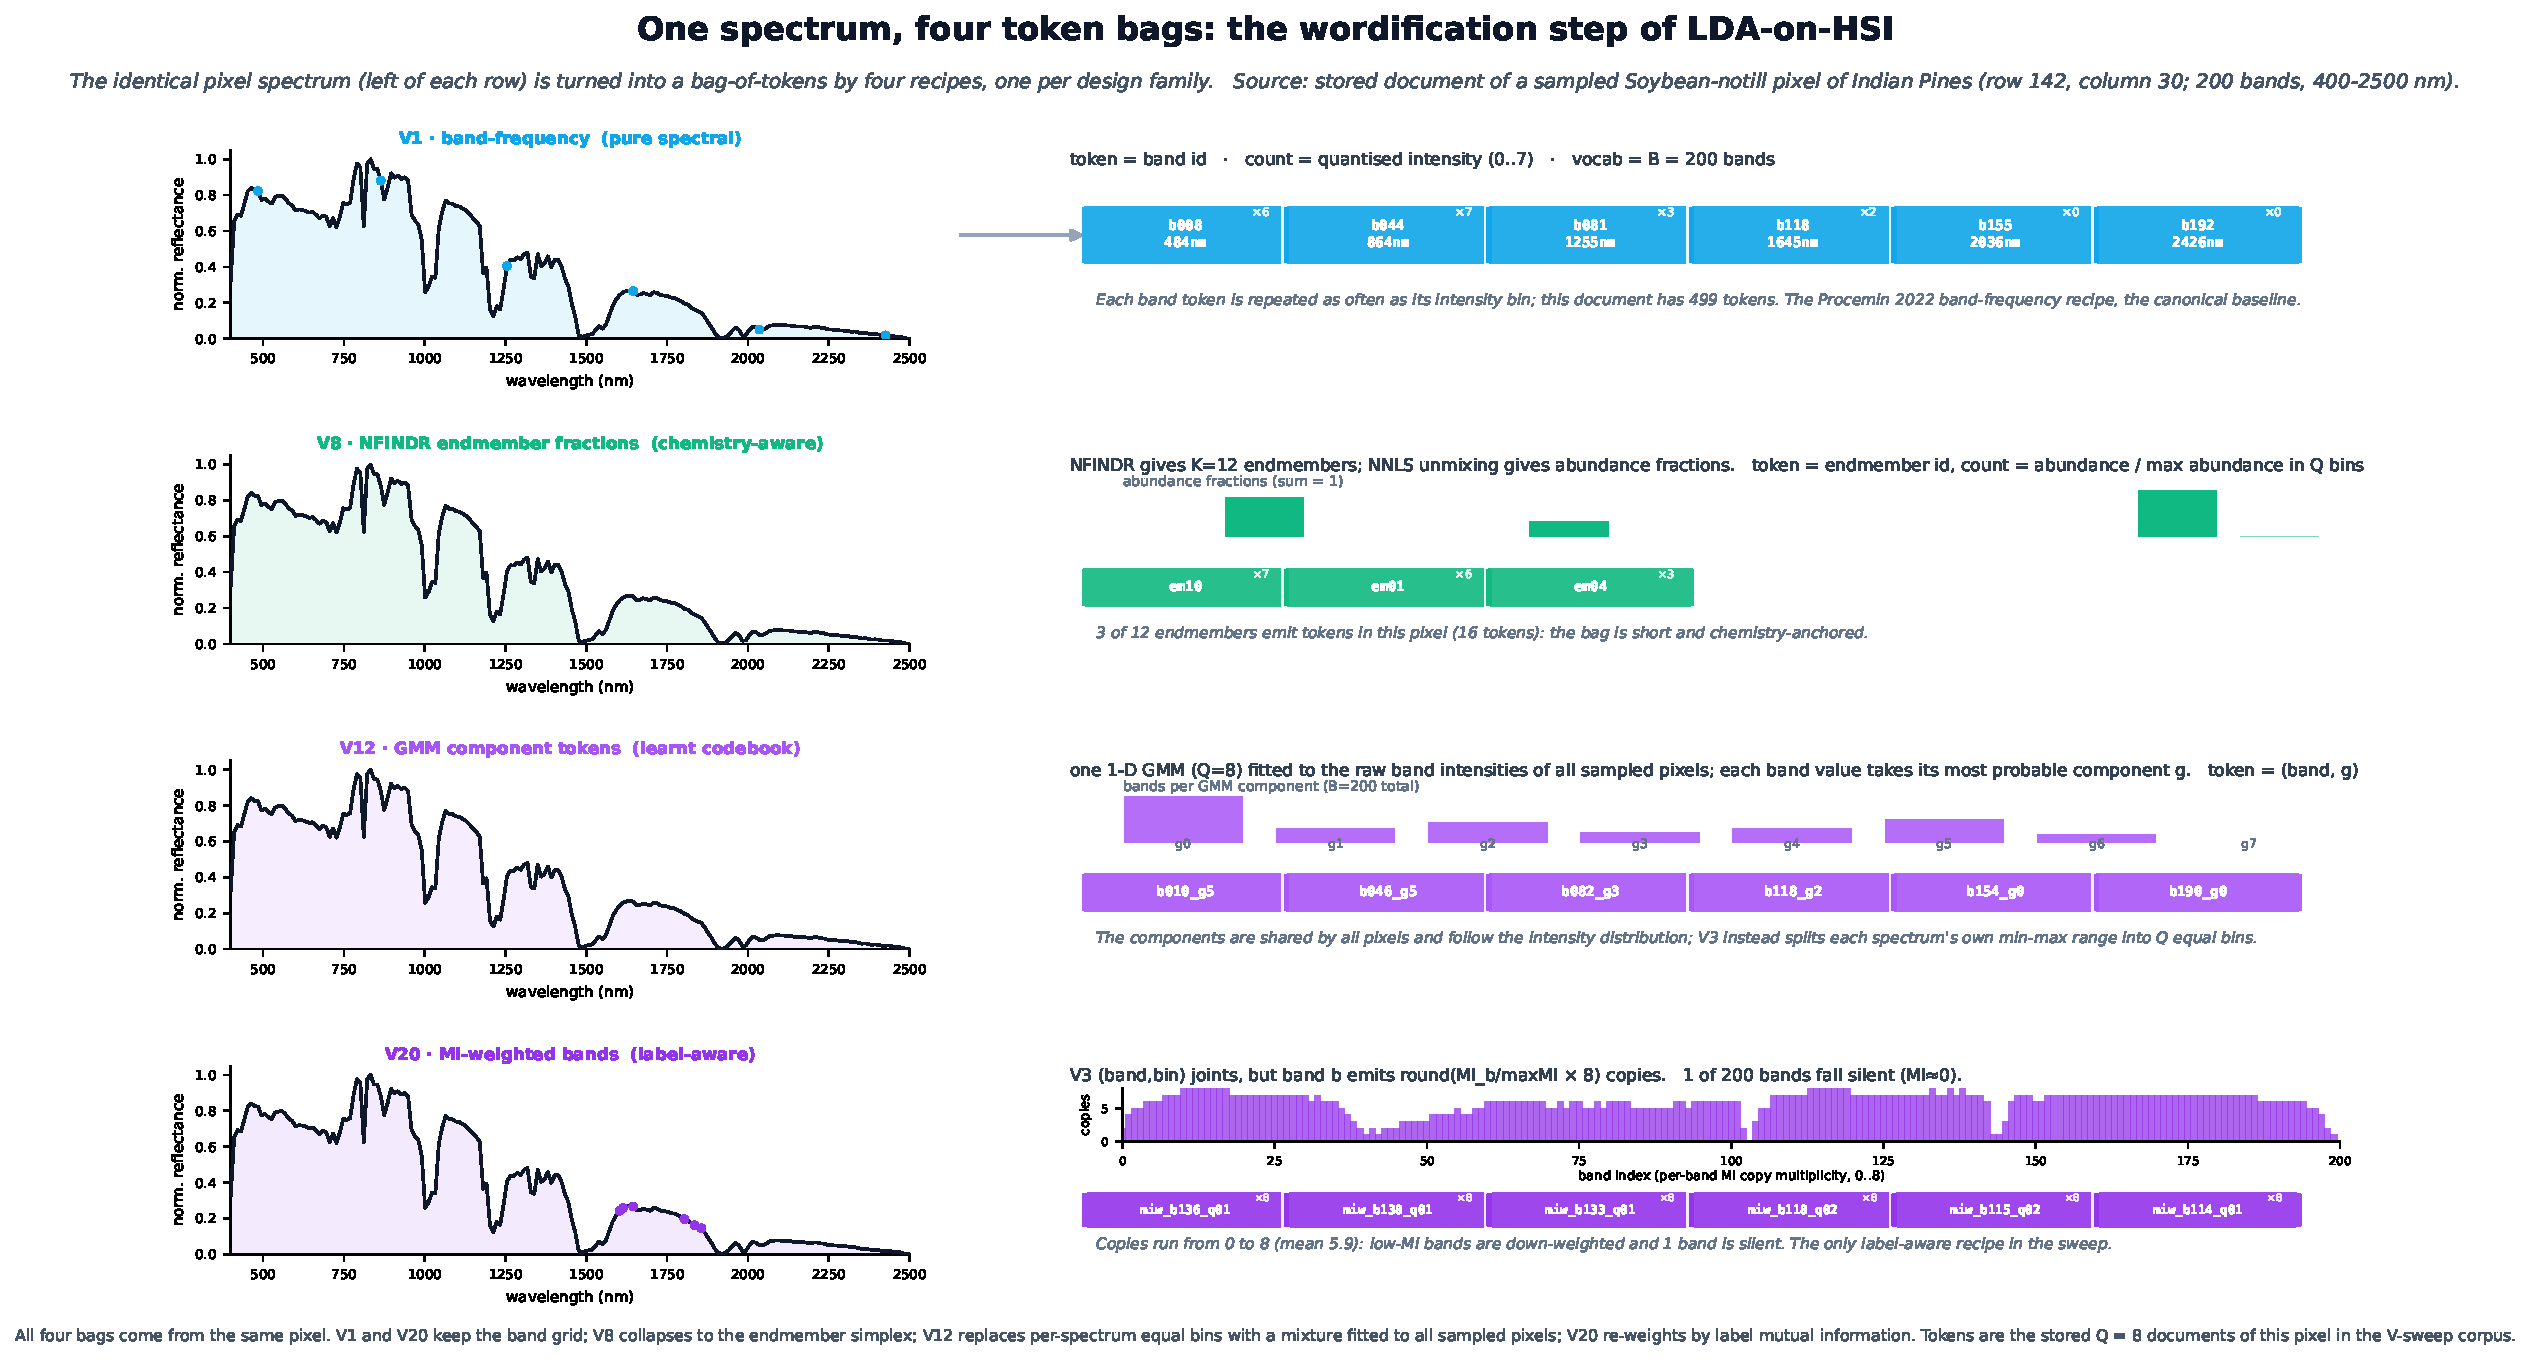
\includegraphics[width=0.95\textwidth]{p3-spectrum-to-tokens.pdf}
\caption{From spectrum to LDA tokens. A normalised pixel spectrum
$x_d \in \mathbb{R}^B$ is mapped to a doc-term count vector $n_d$ by a
recipe-specific $\mathrm{wordify}_V$. The intensity recipes apply the
per-row min--max quantiser $q_b(\cdot)$ of \eqref{eq:quantiser}: V1
emits one band token per band with multiplicity equal to its quantised
intensity \eqref{eq:v1}; V3 emits a single joint (band, bin) token per
band \eqref{eq:v3}; V20 re-emits each V3 token $w_b$ times, with the
per-band weight set by the normalised mutual information of band $b$
with the label \eqref{eq:v20}. The resulting bag of tokens is the
document that LDA \eqref{eq:lda-gen} fits.}
\label{fig:spectrum-to-tokens}
\end{figure*}

\subsection{Per-V K-policy}
\label{subsec:k-policy}
The canonical fit defined in P1 uses
$K = \max(4, \min(12, n_{\text{classes}}))$.
This holds K constant across recipes, which suits recipes with long
documents (V1 averages 450 tokens per document on Indian Pines), but
over-prescribes K when the document length collapses (V7 at
$\le 6$, V9 at 1, V10 at 3, V11 at 4). We therefore set K from the mean
document length $\bar{L}_V$ of each recipe and scene:
\[
K_V = \begin{cases}
K_{\text{P1}}, & \bar{L}_V \ge 8,\\
\mathrm{clip}\big(\mathrm{round}(\bar{L}_V/2),\, 3,\, K_{\text{P1}}\big), & 2.5 \le \bar{L}_V < 8,\\
4, & \bar{L}_V < 2.5,
\end{cases}
\]
where $K_{\text{P1}} = \max(4, \min(12, n_{\text{classes}}))$. This
keeps V1--V6, V8, V12, V14, V18 and V20 at the P1 K, sets V9 to 4, and
reduces V7, V10, V11, V13, V15, V17 and V19 to 3. The one exception is
V10 on Pavia~U, whose 430--860~nm range covers only one of V10's three
band groups: its documents hold a single token and take $K = 4$.

\subsection{Other experimental settings}
The topic backbone is online-variational-Bayes LDA \eqref{eq:lda-gen}
throughout (the cross-backbone HDP / ProdLDA / ETM extensions of
\S\ref{sec:extensions} substitute \eqref{eq:hdp-gen}, \eqref{eq:prodlda-gen}
and \eqref{eq:etm-beta} respectively). All other settings are inherited
verbatim from P1 (the ``Canonical fit'' subsection of that paper):
same stratified-pixel sample, same online-VB hyperparameters, same
five-fold StratifiedKFold, same per-fold LDA refit-no-leakage protocol
and the same per-fold macro-F1, which \S\ref{sec:bayes} summarises with
bootstrap intervals.

% =====================================================================
\section{F-1: classification under V-sweep}\label{sec:results}
% =====================================================================

We follow the F-1 protocol of P1: per-V K-policy, 5-fold
StratifiedKFold (\texttt{random\_state} = 42), per-fold LDA refit with no
test-set leakage at the LDA fit step, two methods reported per cell
(\emph{raw\_logistic} baseline and \emph{topic\_routed\_soft}, the
soft-gated per-topic specialist ensemble from P1). The reported score
is the macro-averaged $F_1$ of \eqref{eq:f1}, computed per fold and
averaged.

\paragraph{V20 leakage caveat} V20 wordification computes per-band
mutual information weights using the full labelled stratified sample
($\text{SAMPLES\_PER\_CLASS} = 220$) before the F-1 5-fold split. The
resulting \texttt{doc\_term} matrix therefore encodes test-fold label
information into the vocabulary structure. The per-fold LDA refit
prevents downstream LDA leakage but does \emph{not} correct the upstream
MI weighting. V20's F-1 macro-F1 should be read with this caveat. Its
six-scene F-1 (0.917 at $Q=8$, 0.916 at $Q=16$ and $Q=32$) does not
exceed that of the label-blind V2 (0.917--0.918) or V8 (0.916--0.917)
at any $Q$, so the leakage produces no visible F-1 advantage, but V20
is not directly comparable with the label-blind recipes on F-1. A
nested protocol (MI weights computed per fold from the training fold
only) removes this leakage; its effect on F-1 is not measured here.
F-2, F-14, F-18 and F-22 use no labels. F-7 has no held-out fold: it is
computed on all sampled pixels, whose labels also set V20's weights, so
V20's F-7 measures the label alignment of a representation built with
those labels.

Table~\ref{tab:f1-full} gives the mean macro-F1 across folds for
\emph{topic\_routed\_soft} on all 6 labelled scenes.

\begin{table*}[ht]
\caption{F-1 mean macro-F1 (topic\_routed\_soft, 5 folds) for V1--V12;
Table~\ref{tab:f1-full19} (Appendix~\ref{app:full-matrix}) gives all
nineteen recipes. Bold = best per scene at full precision (V1 and V6
tie on Salinas-A).}
\label{tab:f1-full}
\centering
\small
\begin{tabular}{lcccccccccccc}
\toprule
Scene & V1 & V2 & V3 & V4 & V5 & V6 & V7 & V8 & V9 & V10 & V11 & V12 \\
\midrule
Botswana          & 0.96 & 0.97 & 0.97 & 0.96 & 0.96 & 0.96 & 0.96 & \textbf{0.97} & 0.96 & 0.97 & 0.96 & 0.97 \\
Indian Pines      & 0.84 & \textbf{0.86} & 0.85 & 0.84 & 0.84 & 0.84 & 0.84 & 0.85 & 0.84 & 0.84 & 0.84 & 0.85 \\
Kennedy SC        & 0.92 & 0.92 & 0.92 & 0.92 & 0.92 & 0.92 & 0.92 & 0.92 & 0.92 & 0.92 & 0.91 & \textbf{0.93} \\
Pavia U           & 0.81 & 0.80 & 0.80 & 0.82 & 0.81 & 0.82 & 0.82 & 0.81 & 0.81 & 0.81 & 0.83 & \textbf{0.83} \\
Salinas-A         & \textbf{0.997} & 0.996 & 0.996 & 0.996 & 0.996 & \textbf{0.997} & 0.996 & 0.995 & 0.996 & 0.996 & 0.996 & 0.996 \\
Salinas           & 0.95 & \textbf{0.96} & 0.95 & 0.95 & 0.95 & 0.95 & 0.95 & 0.95 & 0.95 & 0.95 & 0.95 & 0.95 \\
\midrule
Mean              & 0.9152 & 0.9173 & 0.9153 & 0.9151 & 0.9145 & 0.9135 & 0.9143 & 0.9163 & 0.9143 & 0.9134 & 0.9161 & \textbf{0.9216} \\
\bottomrule
\end{tabular}
\end{table*}

V12 leads with mean macro-F1 = 0.9216; V1 (current canonical) is sixth
at 0.9152. The spread is small (0.0082 across the twelve recipes,
0.0094 across all nineteen): V12 leads on Kennedy SC and Pavia U, V2 on
Indian Pines and Salinas, and V8 on Botswana (by 0.0007 over V3). On
Salinas-A, the easiest scene, V1 and V6 tie at 0.9970 with four
extension recipes, and all nineteen recipes lie within 0.0015.

\S\ref{sec:bayes} compares the recipes with unpaired and paired
bootstrap intervals.

% =====================================================================
\section{F-2: topic--word coherence}\label{sec:f2-results}
% =====================================================================

F-2 is the $c_v$ coherence of \eqref{eq:f2} (NPMI sliding window with
cosine aggregation, top-10 words per topic).
Table~\ref{tab:f2-full} reports the $12 \times 5$ matrix for V1--V12
on five labelled scenes; the Botswana row and the V13--V20 recipes are
reported in Table~\ref{tab:f2-full19} (Appendix~\ref{app:full-matrix}).

\begin{table*}[ht]
\caption{F-2 $c_v$ (top-10 words per topic) for V1--V12 on five
scenes. Bold = best per scene. Sweep run 2026-05-26 on uniform / $Q = 8$.}
\label{tab:f2-full}
\centering
\small
\begin{tabular}{lcccccccccccc}
\toprule
Scene & V1 & V2 & V3 & V4 & V5 & V6 & V7 & V8 & V9 & V10 & V11 & V12 \\
\midrule
Indian Pines     & 0.32 & 0.35 & 0.70 & 0.32 & 0.32 & 0.32 & 0.27 & 0.30 & 0.71 & 0.27 & 0.24 & \textbf{0.79} \\
Kennedy SC       & \textbf{0.97} & 0.76 & 0.93 & 0.81 & 0.93 & 0.79 & 0.37 & 0.52 & 0.72 & 0.53 & 0.25 & 0.89 \\
Pavia U          & 0.91 & 0.43 & 0.96 & 0.59 & 0.40 & 0.58 & 0.27 & 0.21 & 0.70 & 0.32 & 0.22 & \textbf{1.00} \\
Salinas-A        & \textbf{0.96} & 0.35 & 0.92 & 0.32 & 0.32 & 0.81 & 0.32 & 0.38 & 0.71 & 0.23 & 0.21 & 0.88 \\
Salinas          & 0.36 & 0.35 & 0.65 & 0.32 & 0.32 & 0.32 & 0.20 & 0.21 & 0.72 & 0.29 & 0.22 & \textbf{0.84} \\
\bottomrule
\end{tabular}
\end{table*}

V12 (GMM-token) wins F-2 on three of the five scenes; V1 wins on Kennedy
SC and Salinas-A; V3 is competitive everywhere but wins nowhere.

% =====================================================================
\section{F-7: topic--label coupling under V-sweep}
\label{sec:f7-results}
% =====================================================================

F-7 is the topic--label normalised mutual information of
\eqref{eq:f7}, computed between the argmax topic assignment
$\hat{z}_d = \arg\max_k \theta_{dk}$ and the labelled class $y_d$.
Table~\ref{tab:f7-full} reports the $12 \times 5$ matrix for F-7
NMI between the argmax topic assignment and the labelled class.

\begin{table*}[ht]
\caption{F-7 normalised mutual information between argmax topic and
label for V1--V12 on five scenes. Bold = best per scene at full
precision. Sweep run 2026-05-26 on uniform / $Q = 8$.}
\label{tab:f7-full}
\centering
\small
\begin{tabular}{lcccccccccccc}
\toprule
Scene & V1 & V2 & V3 & V4 & V5 & V6 & V7 & V8 & V9 & V10 & V11 & V12 \\
\midrule
Indian Pines     & 0.34 & 0.35 & \textbf{0.43} & 0.25 & 0.20 & 0.25 & 0.16 & 0.43 & 0.10 & 0.08 & 0.25 & 0.42 \\
Kennedy SC       & 0.41 & 0.40 & \textbf{0.54} & 0.32 & 0.25 & 0.34 & 0.20 & 0.17 & 0.11 & 0.17 & 0.22 & 0.51 \\
Pavia U          & 0.47 & 0.38 & 0.55 & 0.38 & 0.14 & 0.43 & 0.23 & 0.54 & 0.02 & 0.00 & 0.21 & \textbf{0.61} \\
Salinas-A        & 0.62 & 0.64 & \textbf{0.68} & 0.37 & 0.56 & 0.33 & 0.16 & 0.52 & 0.20 & 0.28 & 0.42 & 0.55 \\
Salinas          & 0.47 & 0.54 & 0.43 & 0.39 & 0.44 & 0.32 & 0.28 & 0.56 & 0.14 & 0.20 & 0.33 & \textbf{0.64} \\
\bottomrule
\end{tabular}
\end{table*}

Within this 12-recipe view V3 wins F-7 on Kennedy SC, Salinas-A and
Indian Pines (the last by 0.002 over V8, 0.430 against 0.428) and V12
wins on Pavia U and Salinas. In the full 19-recipe sweep
(Appendix~\ref{app:full-matrix}) V20 wins Indian Pines F-7 at 0.44.
\emph{V1 never wins F-7}: on every labelled scene there is at least
one wordification that produces more label-aligned topics. This is
the strongest single-axis result in the sweep and the key
contribution against the V1-canonical assumption of the companion
paper.

% =====================================================================
\section{F-2 and F-7 under the V13--V20 extension}
\label{sec:f-extension-results}
% =====================================================================

Table~\ref{tab:f2-extension} and Table~\ref{tab:f7-extension} restate
F-2 $c_v$ and F-7 normalised MI on a representative subset of recipes
(V1, V3, V12 as the V1--V12 reference points, plus the seven extension
recipes V13--V15 and V17--V20). The full 19-recipe matrix
is reproduced in Appendix~\ref{app:full-matrix}.

\begin{table*}[ht]
\caption{F-2 $c_v$ across the V1--V20 wordification family, restricted
to the V13--V20 extension plus three reference recipes
(V1, V3, V12). Bold = best in this subset; the full-19 winners are
called out in the text. Run 2026-05-28.}
\label{tab:f2-extension}
\centering
\small
\begin{tabular}{lcccccccccc}
\toprule
Scene & V1 & V3 & V12 & V13 & V14 & V15 & V17 & V18 & V19 & V20 \\
\midrule
Indian Pines     & 0.32 & 0.70 & 0.79 & 0.29 & 0.46 & 0.29 & 0.34 & 0.58 & 0.37 & \textbf{0.88} \\
Salinas          & 0.36 & 0.65 & \textbf{0.84} & 0.29 & 0.53 & 0.36 & 0.59 & 0.51 & 0.32 & 0.80 \\
Salinas-A        & \textbf{0.96} & 0.92 & 0.88 & 0.22 & 0.72 & 0.39 & 0.45 & 0.52 & 0.38 & 0.74 \\
Pavia U          & 0.91 & 0.96 & \textbf{1.00} & 0.28 & 0.76 & 0.25 & 0.40 & 0.66 & 0.39 & 0.95 \\
Kennedy SC       & \textbf{0.97} & 0.93 & 0.89 & 0.26 & 0.76 & 0.50 & 0.42 & 0.63 & 0.41 & 0.88 \\
Botswana         & 0.35 & \textbf{0.90} & 0.85 & 0.17 & 0.52 & 0.39 & 0.34 & 0.50 & 0.38 & 0.85 \\
\midrule
mean             & 0.64 & 0.84 & 0.88 & 0.25 & 0.63 & 0.36 & 0.42 & 0.57 & 0.38 & 0.85 \\
\bottomrule
\end{tabular}
\end{table*}

\begin{table*}[ht]
\caption{F-7 NMI across the V1--V20 wordification family, restricted
to the V13--V20 extension plus three reference recipes
(V1, V3, V12). Bold = best in this subset; the full-19 winners are
called out in the text. Run 2026-05-28.}
\label{tab:f7-extension}
\centering
\small
\begin{tabular}{lcccccccccc}
\toprule
Scene & V1 & V3 & V12 & V13 & V14 & V15 & V17 & V18 & V19 & V20 \\
\midrule
Indian Pines     & 0.34 & 0.43 & 0.42 & 0.29 & 0.31 & 0.26 & 0.18 & 0.27 & 0.21 & \textbf{0.44} \\
Salinas          & 0.47 & 0.43 & \textbf{0.64} & 0.35 & 0.51 & 0.28 & 0.17 & 0.50 & 0.35 & 0.47 \\
Salinas-A        & 0.62 & \textbf{0.68} & 0.55 & 0.49 & 0.55 & 0.51 & 0.34 & 0.52 & 0.33 & 0.68 \\
Pavia U          & 0.47 & 0.55 & \textbf{0.61} & 0.22 & 0.49 & 0.28 & 0.21 & 0.52 & 0.36 & 0.54 \\
Kennedy SC       & 0.41 & \textbf{0.54} & 0.51 & 0.31 & 0.43 & 0.29 & 0.21 & 0.28 & 0.25 & 0.52 \\
Botswana         & 0.42 & \textbf{0.52} & 0.46 & 0.21 & 0.44 & 0.25 & 0.19 & 0.47 & 0.21 & 0.47 \\
\midrule
mean             & 0.45 & 0.52 & \textbf{0.53} & 0.31 & 0.46 & 0.31 & 0.22 & 0.43 & 0.29 & 0.52 \\
\bottomrule
\end{tabular}
\end{table*}

\paragraph{V20: mutual-information-weighted bands}
V20 is the cheapest answer to ``why are all bands weighted equally?''
in V3: re-emit each (band, q-bin) token $w_b$ times where
$w_b = \mathrm{round}(\mathrm{MI}_{\mathrm{norm}}(x_b; y) \cdot 8)$.
Per-band MI is estimated once per scene on the labelled stratified
sample (the leakage caveat of \S\ref{sec:results}) with
\path{sklearn.feature_selection.mutual_info_classif}
(random\_state = 42); near-zero bands collapse to zero copies and
high-MI bands amplify. \emph{V20 wins F-2 on Indian Pines (0.88) and
F-7 NMI on Indian Pines (0.44)}, places second to V3 on Salinas-A F-7
(0.68 tie), and matches V12 within $0.02$ NMI mean. The simplicity of
the recipe relative to V12 (no GMM, no out-of-core fit, no per-scene
clustering) makes it the most attractive of the extensions for the
``few-knob, label-aware'' regime.

\paragraph{V18: graph-Laplacian eigenvector tokens}
V18 builds a $K=10$ nearest-neighbour cosine-affinity graph over the
sampled pixels, computes the symmetric-normalised Laplacian
$L = I - D^{-1/2}AD^{-1/2}$, extracts the first 16 eigenvectors via
\texttt{scipy.sparse.linalg.eigsh} (sigma-magnitude solver),
percentile-bins each eigenvector axis into $Q = 8$ bins, and emits
one (eigenvector\_id, bin) token per axis per pixel. The intuition is
that low-frequency Laplacian eigenvectors carry global manifold
structure that LDA can latch onto. The mean F-7 NMI of 0.43 places
V18 third among the extension recipes (behind V20 0.52 and V14 0.46) and
\emph{V18 produces the most coherent topics on Pavia U among the
unsupervised structure-aware extension recipes} (V13, V17, V18, V19; $c_v = 0.66$). We read V18 topics as
contiguous manifold regions rather than band-signature templates, a
reading these runs do not test.

\paragraph{V14: continuous-wavelet (Morlet) tokens}
V14 emits top-16 magnitude cells from a 16-log-scale, 8-position-bucket
CWT-Morlet decomposition of the spectrum. It is the multi-scale
analogue of V6 (Db4 DWT). V14 places second among the extension recipes on
F-7 mean (0.46) and produces the second-highest $c_v$ on the extension
subset on Pavia U and Kennedy SC. V14 outperforms V6, the
discrete-wavelet recipe, on four of the six scenes (mean $c_v$ 0.63
against 0.53).

\paragraph{V13 / V17 / V19: underperformers and the cost of
expressiveness}
V13 (VQ-VAE codebook), V17 (sparse-coding dictionary), and V19 (UMAP
coordinates) all underperform the V1/V3/V12 reference on F-2 and F-7.
V13's mean F-2 of 0.25 is the second lowest in the nineteen-recipe
sweep, after V11 (0.23). A plausible reason is that the jointly
trained encoder, codebook and decoder (straight-through estimator)
produce compact codes suited to reconstruction rather than to the
topic-as-mixture-of-tokens assumption of LDA. V17 has the opposite
profile: a 512-token vocabulary (64 atoms $\times$ 8 abundance bins)
with 3.4 tokens per document on Indian Pines (at most 8 non-zero
coefficients per pixel), a sparsity under which LDA finds few coherent
topics. V19's
3-coordinate tokens are too few, and the per-axis percentile binning
produces tokens that are abstract (``UMAP-d0 q03'') and cannot align
with class-specific spectral signatures. The takeaway is that
expressive learnt representations need not produce LDA-friendly token
distributions; the recipe must respect the bag-of-tokens assumption.

\paragraph{V15: spectral-index tokens}
V15 emits NDVI/MNDWI/NBR/NDSI/EVI/SAVI per pixel, with each index
q-binned. V15 places below V14 on every axis (F-2 mean 0.36 vs 0.63;
F-7 mean 0.31 vs 0.46) but is the only recipe whose token names map
to a published remote-sensing semantic: in a topic-as-region
interpretation, a topic dominated by ``NDVI q05--q07'' is unambiguously
vegetated. V15 should therefore be regarded as a \emph{semantic
baseline} rather than as a performance recipe.

% =====================================================================
\section{Bootstrap comparison on F-1}\label{sec:bayes}
% =====================================================================

We summarise each recipe's mean macro-F1 with a bootstrap percentile
interval ($B = 5000$ resamples of its 30 per-fold scores,
$\mathrm{random\_state} = 42$; Table~\ref{tab:bootstrap}).

\begin{table}[ht]
\caption{Per-recipe bootstrap mean and 94\% percentile interval
(3\% and 97\% quantiles of the resampled means) of the F-1 macro-F1,
topic\_routed\_soft, V1--V12.}
\label{tab:bootstrap}
\centering
\small
\begin{tabular}{lcc}
\toprule
Recipe & bootstrap mean & 94\% interval \\
\midrule
V12  & 0.9217 & [0.9005, 0.9424] \\
V2   & 0.9171 & [0.8932, 0.9395] \\
V11  & 0.9163 & [0.8939, 0.9375] \\
V8   & 0.9161 & [0.8933, 0.9386] \\
V3   & 0.9156 & [0.8922, 0.9381] \\
V1   & 0.9153 & [0.8924, 0.9375] \\
V4   & 0.9149 & [0.8927, 0.9367] \\
V5   & 0.9143 & [0.8902, 0.9367] \\
V9   & 0.9141 & [0.8905, 0.9360] \\
V7   & 0.9140 & [0.8920, 0.9354] \\
V10  & 0.9133 & [0.8881, 0.9364] \\
V6   & 0.9132 & [0.8893, 0.9362] \\
\bottomrule
\end{tabular}
\end{table}

The spread between V12 (best) and V6 (worst) is $0.0085$, and every
recipe's interval contains every other recipe's mean. These unpaired
intervals are wide because the 30 scores of a recipe mix six scenes
whose F-1 runs from 0.80 on Pavia~U to 0.997 on Salinas-A, so their
overlap does not show that the recipes perform alike. All recipes share
the stratified sample and the fold split of each scene, so their fold
scores pair. Over the 30 paired (scene, fold) cells, V12 exceeds each
of the other eighteen recipes by 0.004 to 0.009 on average (V1:
$+0.0064$, 94\% paired bootstrap interval $0.0032$ to $0.0100$), and the
interval excludes zero for every recipe except V2 ($+0.0043$, $-0.0001$
to $+0.0095$). The five folds of a scene share training pixels, so
these paired intervals are narrower than a resampling of independent
cells would give. On F-1 the recipes therefore differ consistently but
by less than 0.01. F-2 and F-7 separate them by far more: the spread
between the best and worst recipe mean over the five scenes of
Tables \ref{tab:f2-full} and \ref{tab:f7-full} is 0.65 on F-2 (V12
against V11) and 0.43 on F-7 (V12 against V9). The paired comparison is
computed from the archived per-fold records by
\path{scripts/f1_paired_bootstrap.py} of the manuscript repository
\url{https://github.com/fsantibanezleal/CAOS_LDA_HSI_Paper}.

% =====================================================================
\section{The joint result matrix}\label{sec:matrix}
% =====================================================================

Across F-1, F-2 and F-7 on the six labelled scenes, each recipe's win
count is:

\begin{table}[ht]
\caption{Per-axis win count for each recipe over the nineteen-recipe
sweep on the six labelled scenes (F-1: topic\_routed\_soft macro-F1).
The Salinas-A F-1 cell is a six-way tie at 0.9970 (V1, V6, V13, V14,
V18, V20) and is not counted. Total = sum across F-1, F-2 and F-7.}
\label{tab:wincount}
\centering
\small
\begin{tabular}{lrrrr}
\toprule
Recipe & F-1 wins & F-2 wins & F-7 wins & Total \\
\midrule
V12 & 2 & 2 & 2 & \textbf{6} \\
V20 & 0 & 1 & 1 & 2 \\
V3  & 0 & 1 & 2 & 3 \\
V1  & 0 & 2 & 0 & 2 \\
V2  & 2 & 0 & 0 & 2 \\
V8  & 1 & 0 & 1 & 2 \\
\bottomrule
\end{tabular}
\end{table}

V12 is the most consistent winner across the three axes, but the
nineteen-recipe sweep redistributes the F-2 and F-7 wins of the
twelve-recipe view. V20 captures one F-2 win (Indian Pines, $0.88$)
and one F-7 win (Indian Pines, $0.44$); on Indian Pines F-7 four
recipes lie within 0.018 NMI (Table~\ref{tab:f7-full19}: V20 0.442,
V3 0.430, V8 0.428, V12 0.424). On F-7, V3 keeps its Kennedy SC and
Salinas-A wins and loses Indian Pines, its third twelve-recipe win, to
V20. V1 (current canonical) wins F-2 on Kennedy SC and Salinas-A,
shares the six-way F-1 tie on Salinas-A, and never wins F-7. The
spread between V12, V3 and V20 on F-7 mean is only $0.014$ NMI: a flat
top, not a sharp peak.

% =====================================================================
\section{Extension axes F-13, F-14, F-17, F-18, F-22 and backbone factorial}
\label{sec:extensions}
% =====================================================================

Five further axes extend the framework beyond F-1--F-12, and a
backbone factorial repeats F-2 and F-7 under three alternative topic
models. Each is described briefly here; the full per-recipe, per-scene tables and the
code that builds them are released with the code repository (Data
availability). The quantiser sweep $Q \in \{8, 16, 32\}$ of F-2 and
F-7 under LDA is shown in Fig.~\ref{fig:q-sensitivity} (all nineteen
recipes) and Fig.~\ref{fig:per-scene-q-winners} (per-scene F-7
winners); Fig.~\ref{fig:radar} profiles six recipes over the eight
axes, and Fig.~\ref{fig:corr} gives the rank correlation between the
axes.

\textbf{F-13 SHAP attribution.} For every (V, scene) we attribute
$\theta_{d,k}$ to recipe-specific tokens using SHAP's KernelExplainer
on a closed-form posterior and report the top-8 tokens per topic by
mean absolute SHAP. These attributions are archived (Data availability)
and not analysed in this paper.

\textbf{F-14 repetitiveness.} Mean off-diagonal top-10 Jaccard between
topics \eqref{eq:f14}. Lower is better. Per-recipe mean across six
scenes:
V9 = 0.000, V17 = 0.003, V7 = 0.009, V12 = 0.009, V3 = 0.012;
V1 = 0.200 (mid-pack); V6 = 0.738, V8 = 0.868 and V2 = 1.000. V2 and
V8 meet the vocabulary criterion stated under F-18 below (at most 12
word types), so any two of their top-10 sets share at least 8 tokens
and their F-14 values are high by construction; V6's vocabulary has
131--230 word types, of which 14--58 occur in the documents of a
scene.

\textbf{F-17 cross-scene transfer.} Fit $\phi$ on scene S1, transform
S2's documents, compute F-7 NMI on the target. Only vocab-portable
recipes (V2, V10, V11) qualify. V2 transfers best at 0.32 mean NMI;
V11 0.19; V10 0.10.

\textbf{F-18 reliability.} Greene et al.\ (2014) protocol \cite{greene2014topics}:
Hungarian-matched \cite{kuhn1955hungarian} top-10 indicator cosine
similarity across reseed pairs (seeds 42--46), as in \eqref{eq:f18}.
Per-recipe mean fraction-above-0.7 across the six labelled scenes:

\begin{center}
\scriptsize
\setlength{\tabcolsep}{2pt}
\begin{tabular}{lcccccccccccc}
\toprule
& V1 & V2 & V3 & V4 & V5 & V6 & V7 & V8 & V9 & V10 & V11 & V12 \\
\midrule
F-18 & 0.25 & \emph{1.00} & 0.19 & 0.20 & 0.15 & 0.95 & 0.15 & \emph{1.00} & 0.00 & 0.54 & 0.28 & \textbf{0.14} \\
\bottomrule
\end{tabular}
\end{center}

\emph{Italic} marks the recipes that meet the vocabulary criterion used
throughout this paper: a vocabulary of at most 12 word types. Any two
top-10 sets drawn from at most 12 word types share at least 8 tokens,
so every Hungarian-matched pair has cosine at least 0.8 and passes the
0.7 threshold by construction, whatever the fits. V2 (8 word types at
$Q=8$) and V8, whose vocabulary is its set of NFINDR endmembers
($K_e = 12$ word types on four scenes, 9 on Pavia~U and 6 on
Salinas-A), meet the criterion on every scene, so their F-18 values
measure the vocabulary size rather than reseed reliability. V6
(131--230 word types) does not meet it, and its 0.95 is not flagged.
The \textbf{bold} V12 marks
the recipe that leads F-2 and F-7 at $Q=8$ (its F-1 lead is below
0.01) but loses F-14 to V9, loses F-22 to V20 (V20 26.3 vs V12 24.5),
and loses F-18 to every recipe except V9. V12's flexibility is
seed-sensitive.

\paragraph{The reliability--informativeness tradeoff}
V12, V3, V7, V5, V4 all sit in the 0.14--0.20 range: informative
but seed-sensitive. V1 (current canonical) at 0.25 is the most
reliable of the per-band recipes (V1, V3, V4, V5, V12), whose
vocabularies have $B$ or $B \cdot Q$ word types; V6 (0.95), V10 (0.54)
and V11 (0.28) score higher without meeting the vocabulary criterion.
This is the strongest argument for V1 retaining
its canonical status \emph{even though V12 leads F-2 and F-7}: V1 is
the most reliable of the per-band wordifications.

\paragraph{V20 falls on the V12 side of the reliability axis}
The extended F-18 sweep with the label-aware recipe gives V20 a
fraction above 0.7 of $0.22$ at $Q=8$ and at $Q=16$ (mean matched
cosine $0.451$ and $0.450$) across the six labelled scenes, inside the
0.14--0.25 band of the per-band recipes V12, V3, V4 and V1, despite
V20's strong F-2 / F-7 / F-22 performance. A possible reason, which
these runs do not test, is that the down-weighted low-MI bands leave
parts of the topic--word matrix flat, so different LDA seeds refine the
high-MI bands differently. \textbf{V8 (NFINDR endmember-fraction)}
reaches a mean matched cosine of $0.957$ ($Q=8$) and $0.962$ ($Q=16$),
but it meets the vocabulary criterion: its top-10 sets cover all or
nearly all of its 6--12 endmember tokens, so every matched pair has
cosine at least 0.8 whatever the fits, and these values do not measure
reseed reliability.
V8's cross-backbone portability (top-3 mean F-7 NMI across LDA / HDP /
ProdLDA / ETM, \S\ref{subsec:backbone-f7}) does not rest on F-18.

\textbf{F-22 counterfactual.} The minimum-$L_1$ token perturbation
that flips $\arg\max_k \theta_k(n_d)$, as defined in \eqref{eq:f22};
we solve it by coordinate-descent search capped at
$\text{MAX\_STEPS} = 50$ token-flips. Cells where every sampled
document fails to flip persist with the sentinel value $50$ rather
than being dropped. Higher = more robust topic boundary. Per-recipe
mean of the per-scene medians across the 19-recipe sweep:

\begin{center}
\scriptsize
\setlength{\tabcolsep}{3pt}
\begin{tabular}{l*{10}{c}}
\toprule
recipe & V1 & V2 & V3 & V4 & V5 & V6 & V7 & V8 & V9 & V10 \\
\midrule
$L_1$ & 6.1 & 7.8 & 23.5 & 2.5 & 2.5 & 1.9 & 5.2 & 3.6 & 1.0 & 1.2 \\
\midrule
recipe & V11 & V12 & V13 & V14 & V15 & V17 & V18 & V19 & V20 & \\
\midrule
$L_1$ & 3.3 & 24.5 & 2.7 & 7.7 & 4.0 & 2.6 & 3.7 & 2.1 & \textbf{26.3} & \\
\bottomrule
\end{tabular}
\end{center}

\textbf{V20 has the highest F-22} in the sweep
($L_1 = 26.3$), surpassing V12 (24.5), the most robust of V1--V12,
and the joint (band, q-bin) vocabulary V3 (23.5). On three scenes (Salinas-A,
Pavia U, Botswana) every sampled document under V20 failed to flip
within 50 perturbations; the sentinel value $50$ caps that
observation. F-22 counts unit token changes, so it grows with the
document length: a V20 document holds 1187 tokens on Indian Pines
against 200 for V3 and V12 (each band repeated $w_b$ times, 5.9 on
average), and part of V20's lead may reflect that scale rather than a
more robust topic boundary. V9 (one token per document) flips at the
first perturbation.

\paragraph{F-22 Q-trajectory} Re-running the four top contenders at
$Q \in \{8, 16, 32\}$ reveals a non-monotonic peak for V20 at $Q=16$
($L_1 = 41.83$, $+59\%$ over $Q=8$, with five of the six scenes at the
sentinel 50), falling back to $26.17$ at $Q=32$. V12 leads at $Q=32$
($L_1 = 30.00$, after $24.50$ at $Q=8$ and $20.67$ at $Q=16$). V8 is the
only top contender whose $L_1$ rises monotonically with $Q$ ($3.58$,
$9.58$ and $20.25$ at $Q = 8$, $16$ and $32$), roughly in proportion to
$Q$: its counts are NNLS abundances quantised to $Q$ levels, so the
rise may reflect the count scale rather than preserved discriminative
structure.

\begin{figure*}[!t]
\centering
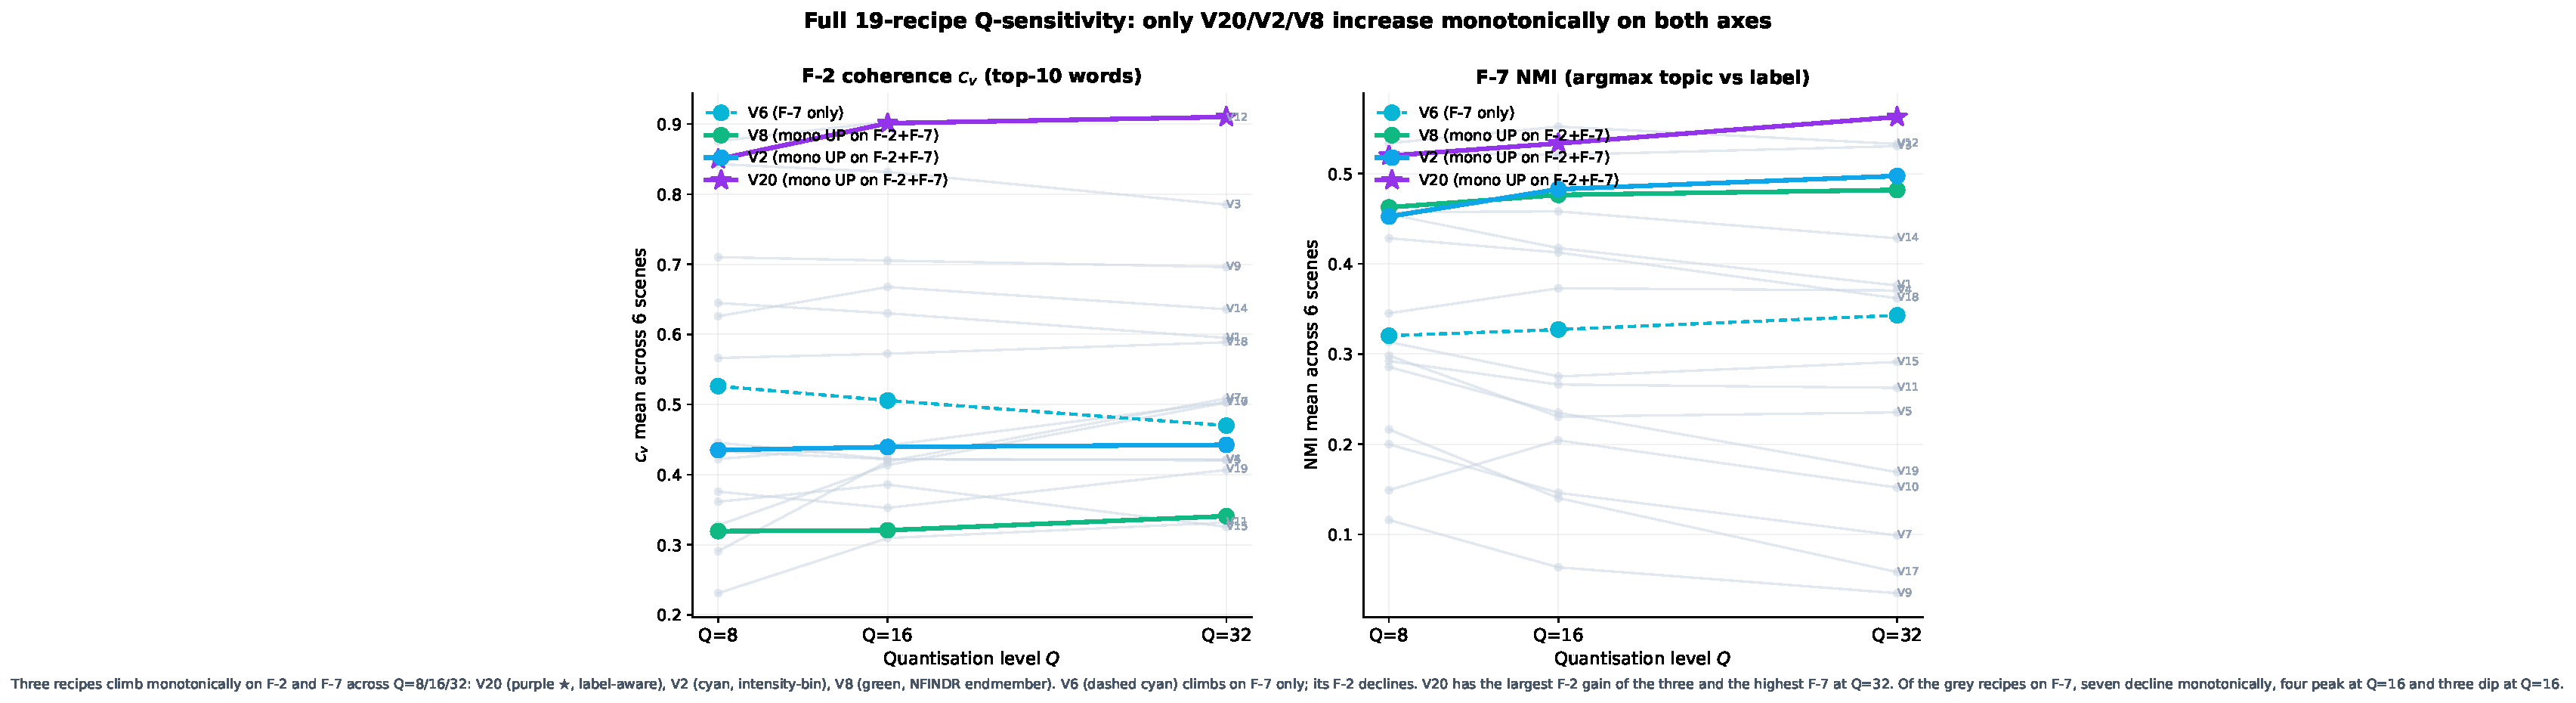
\includegraphics[width=0.95\textwidth]{q-sensitivity-all19.pdf}
\caption{Full 19-recipe Q-sensitivity under LDA. Both F-2 $c_v$ and
F-7 NMI plotted across $Q \in \{8, 16, 32\}$ for every recipe (V13
is excluded because it is insensitive to $Q$). \textbf{Three recipes climb monotonically
on both F-2 and F-7}: V20 (purple, $\star$, label-aware), V2 (cyan,
intensity-bin), V8 (green, NFINDR endmember). V6 (dashed cyan) is
monotonic on F-7 only. The remaining 14 recipes are grey: on F-7,
seven decline monotonically (V1, V7, V9, V11, V17, V18, V19), four
peak at $Q=16$ (V4, V10, V12, V14) and three dip at $Q=16$ (V3, V5,
V15). Of the three rising recipes, V20 has the largest F-2 gain
(+0.060); its F-7 gain is +0.043 (V2: +0.045). V20 has the highest
absolute F-7 at $Q=32$ (0.563); on F-2 it ties V12 (0.910 vs 0.909).
V20 is the only \emph{label-aware} recipe in the monotonic-improvement
family.}
\label{fig:q-sensitivity}
\end{figure*}

\begin{figure*}[!t]
\centering
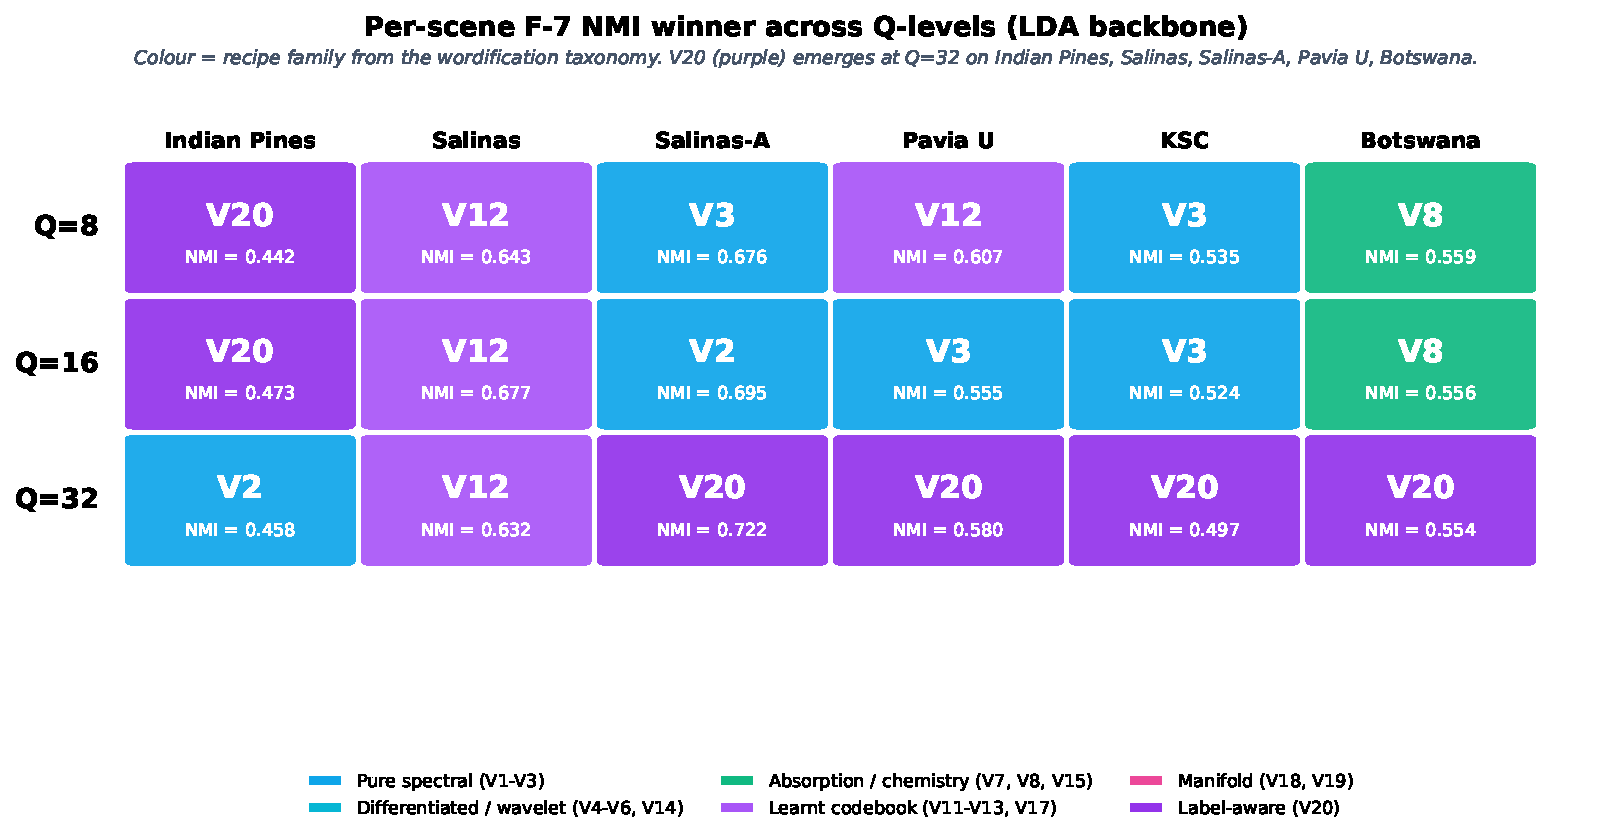
\includegraphics[width=0.95\textwidth]{per-scene-q-winners.pdf}
\caption{Per-scene F-7 NMI winner under LDA at each quantisation
level. V20 dominance scales with Q: at $Q=8$ V20 wins only on
Indian Pines (1/6 scenes), at $Q=16$ V20 still wins only Indian
Pines (1/6), and at $Q=32$ V20 wins four of six scenes
(Salinas-A, Pavia U, KSC, Botswana). The jump from 1/6 to 4/6
between Q=16 and Q=32 is the sharpest single Q-step gain in the
sweep. The Q=8 row gives V12 two wins, V3 two, V20 one and V8 one;
V12 falls to one win at $Q=16$ and at $Q=32$, and V3 keeps two at
$Q=16$ and has none at $Q=32$.
The rise is consistent with V20's per-band MI re-weighting gaining
from finer intensity bins.}
\label{fig:per-scene-q-winners}
\end{figure*}

\begin{figure*}[!t]
\centering
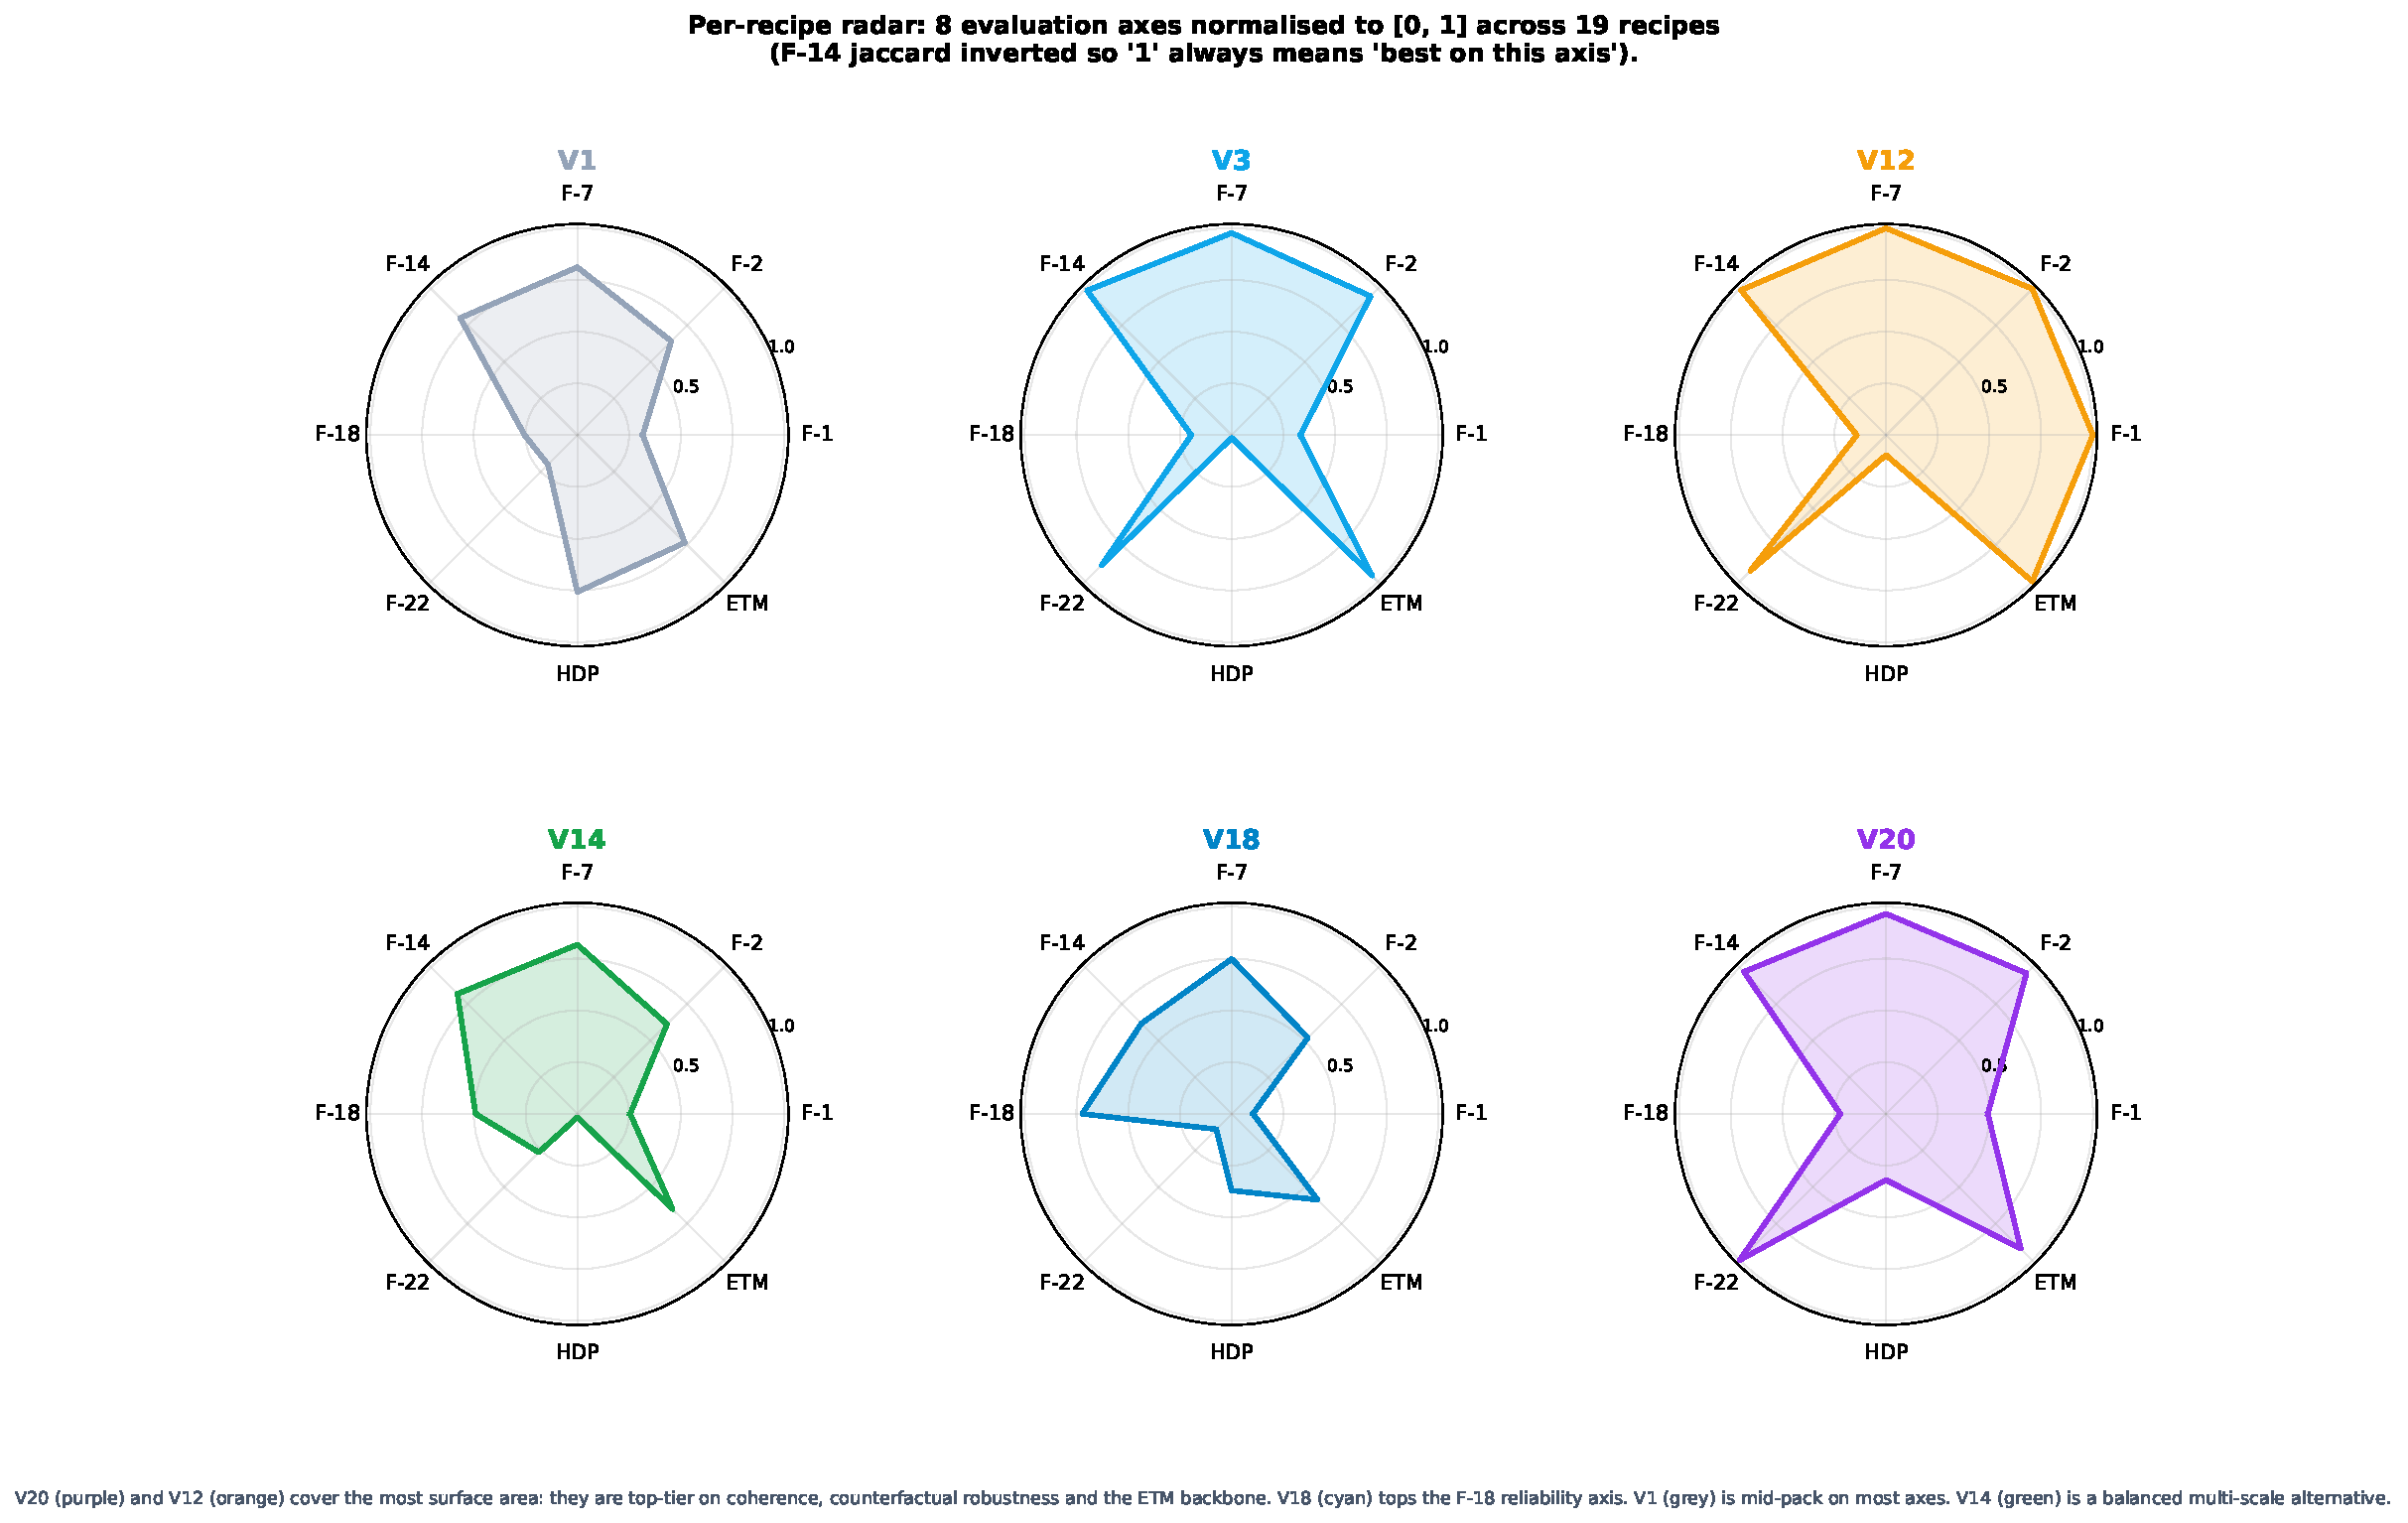
\includegraphics[width=0.95\textwidth]{p3-radar-top-recipes.pdf}
\caption{Per-recipe radar across the eight evaluation axes, normalised
to $[0, 1]$ across the 19-recipe set. F-14 (jaccard) is sign-inverted
so ``1'' always means ``best on this axis''. V20 (purple) and V12
(orange) cover the most surface area; V18 (cyan) has the highest F-18
of the six recipes shown; V1 (grey) is mid-pack on most axes.}
\label{fig:radar}
\end{figure*}

\begin{figure*}[!t]
\centering
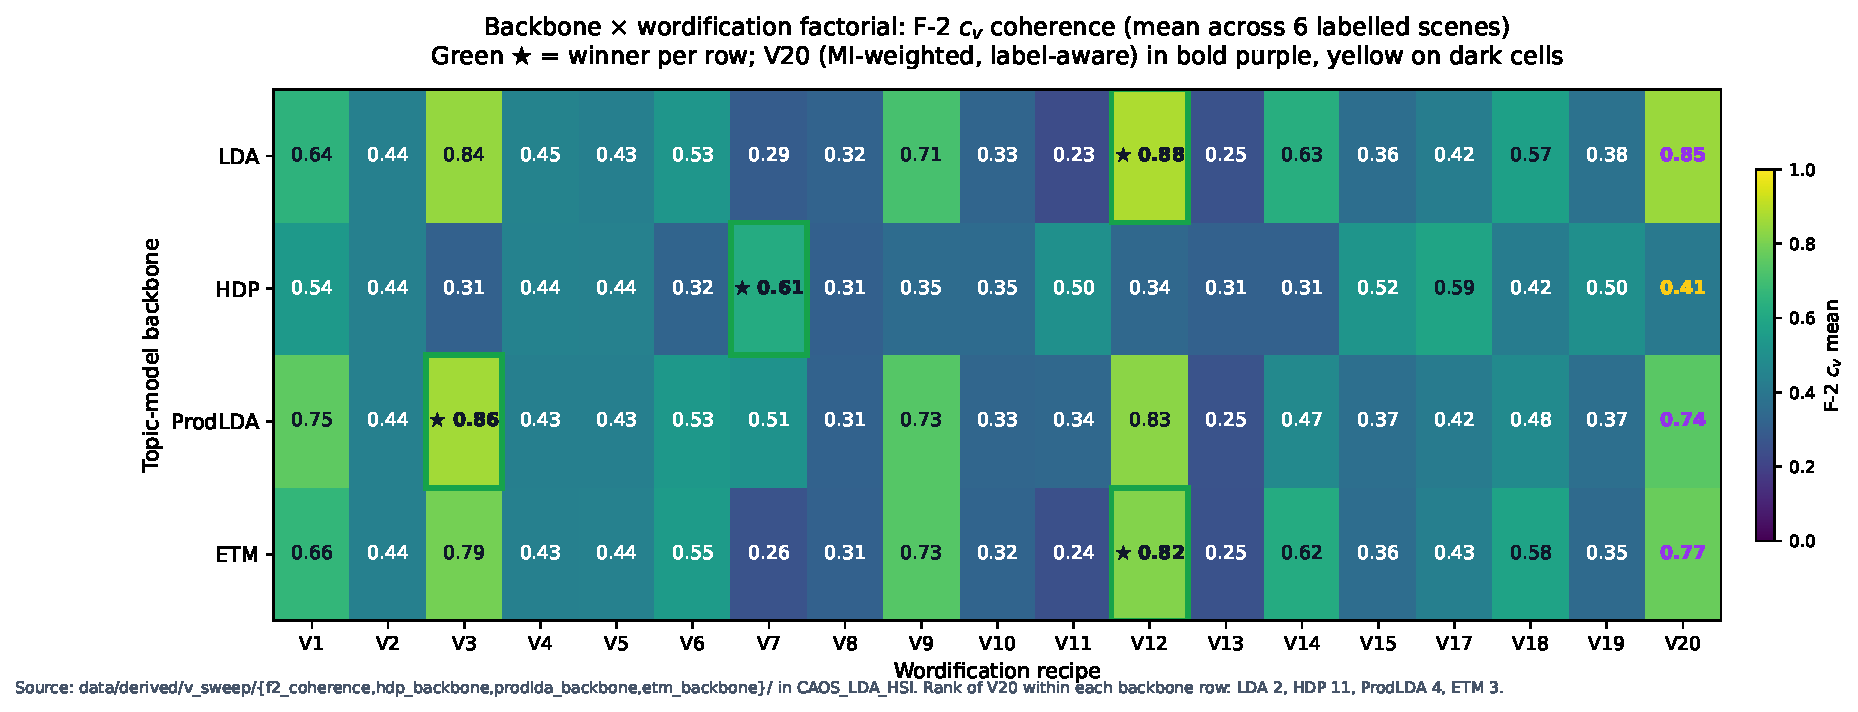
\includegraphics[width=0.99\textwidth]{p4-backbone-factorial.pdf}
\caption{Backbone $\times$ wordification factorial. Each cell shows
the mean F-2 $c_v$ across the six labelled scenes for one
(backbone, recipe) pair; one row per backbone, recipes in index
order. Green border + $\star$ = per-backbone winner; V20 (the
label-aware recipe) is labelled in bold purple (yellow on dark cells),
and the footer gives its rank within each row (LDA 2, HDP 11, ProdLDA
4, ETM 3; under HDP, V20 is tenth without the V15 cell noted at the
end of this caption). No recipe dominates every backbone: LDA and ETM pick V12,
with V3 and V20 close behind; HDP picks V7 (sparse absorption tokens);
ProdLDA picks V3. The HDP cell for V15 (0.52) was computed on the
stored V15 wordification that holds the $Q=32$ vocabulary (192 tokens;
96 on Pavia~U); every other V15 value at $Q=8$ in this paper uses the
$Q=8$ vocabulary (48 tokens; 24 on Pavia~U).}
\label{fig:backbone-factorial}
\end{figure*}

\textbf{Backbone factorial: HDP.} The first alternative backbone of
the factorial covers the same 114 cells (nineteen recipes on the six
labelled scenes, Fig.~\ref{fig:backbone-factorial}), with gensim's
Hierarchical Dirichlet Process in place of fixed-K LDA. For five
representative recipes, the per-recipe ranking on F-2 $c_v$
(six-scene means, as in Fig.~\ref{fig:backbone-factorial})
\emph{inverts}:

\begin{center}
\small
\begin{tabular}{lc|lc}
\toprule
LDA backbone & $c_v$ mean & HDP backbone & $c_v$ mean \\
\midrule
V12 & \textbf{0.876} & V7  & \textbf{0.615} \\
V3  & 0.843 & V1  & 0.540 \\
V1  & 0.645 & V11 & 0.501 \\
V7  & 0.291 & V12 & 0.337 \\
V11 & 0.231 & V3  & 0.311 \\
\bottomrule
\end{tabular}
\end{center}

Under LDA the dense GMM-token vocabulary of V12 has the most coherent
topics; under HDP, V7 (at most six absorption-feature tokens per pixel)
leads. The HDP result is consistent with the truncated
Dirichlet-process prior favouring recipes whose few tokens each carry
semantic weight, a hypothesis these runs do not test.
\textbf{This inversion is the cleanest evidence that the
wordification ranking depends on the backbone, which motivates the
factorial study.}

% =====================================================================
\subsection{F-7 NMI across the four backbones}
\label{subsec:backbone-f7}
% =====================================================================

The backbone factorial above reports F-2 $c_v$ only;
Table~\ref{tab:f7-4backbone} adds F-7 NMI under each non-LDA backbone.

\begin{table}[ht]
\caption{F-7 NMI mean across the six labelled scenes, top-12 recipes
$\times$ four topic-model backbones (full sweep, 456/456 cells).
Bold = per-backbone winner. Recipes sorted by 4-backbone mean. LDA uses
the per-recipe K of \S\ref{subsec:k-policy}; the F-7 runs of ProdLDA and
ETM use $K = K_{\text{P1}}$ for every recipe, and HDP truncates at 20
topics.}
\label{tab:f7-4backbone}
\centering
\scriptsize
\setlength{\tabcolsep}{4pt}
\begin{tabular}{lccccc}
\toprule
Recipe & LDA & HDP & ProdLDA & ETM & \textbf{Mean} \\
\midrule
\textbf{V8}  (NFINDR)       & 0.463 & 0.451 & \textbf{0.328} & 0.482 & \textbf{0.431} \\
V20 (MI-weighted)           & 0.520 & 0.356 & 0.221 & 0.490 & 0.397 \\
V2  (intensity-bin)         & 0.453 & 0.347 & 0.324 & 0.456 & 0.395 \\
V11 (product quantisation)  & 0.292 & \textbf{0.571} & 0.088 & \textbf{0.530} & 0.370 \\
V12 (GMM-token)             & \textbf{0.534} & 0.220 & 0.238 & 0.488 & 0.370 \\
V3  (joint band-bin)        & 0.524 & 0.200 & 0.169 & 0.443 & 0.334 \\
V19 (UMAP coord)            & 0.286 & 0.530 & 0.051 & 0.394 & 0.315 \\
V15 (spectral indices)      & 0.313 & 0.438 & 0.058 & 0.449 & 0.315 \\
V13 (VQ-VAE)                & 0.311 & 0.399 & 0.113 & 0.406 & 0.307 \\
V14 (CWT-Morlet)            & 0.457 & 0.220 & 0.114 & 0.430 & 0.306 \\
V18 (graph-Laplacian)       & 0.428 & 0.198 & 0.080 & 0.330 & 0.259 \\
V1  (band-frequency)        & 0.455 & 0.081 & 0.091 & 0.381 & 0.252 \\
\bottomrule
\end{tabular}
\end{table}

\paragraph{Degenerate cross-backbone fits}
The 4-backbone $\times$ 19-recipe $\times$ 6-scene Q=8 factorial
contains a non-trivial number of degenerate cells (F-7 below 0.01, an
argmax topic that carries no label information): LDA 1/114, ETM 1/114,
but \textbf{HDP 25/114 (22\%)} and \textbf{ProdLDA 41/114 (36\%)}. For
HDP, 22 of the 25 are on V1, V4, V5 and V6, the recipes for which HDP
keeps between 1.2 and 2.2 effective topics (six-scene means of the F-2
runs); across the nineteen recipes HDP's F-7 follows the number of
topics it keeps (Spearman $\rho = 0.59$). The cross-backbone mean
reported in the table above averages these zeros together with the
other fits.

Excluding zero cells from the per-backbone means yields V8 0.431
(unchanged, since V8 has no degenerate cells), V20 0.408 ($+0.011$, one
ProdLDA zero on Indian Pines), V11 0.381 ($+0.011$), V12 0.393
($+0.023$). V8 retains cross-backbone leadership under either
treatment of zeros. The F-7 value of every (backbone, recipe, scene)
cell is archived in the code repository.

\textbf{V8 (NFINDR endmember-fraction)} is the most
cross-backbone-consistent recipe at mean F-7 NMI $= 0.431$; it lands top-5 under
every backbone, winning outright only under ProdLDA, and shares with V2
the smallest standard deviation across the four backbones
($\sigma = 0.06$ for both). V20
is the second-most consistent at $0.397$, retaining LDA strength
($0.520$) and tying V12 on ETM ($0.490$ vs $0.488$; V11 leads ETM at
$0.530$). V11 (product
quantisation, vocab $M K_s = 32$) wins HDP and ETM outright but
collapses under ProdLDA (0.088) and ranks low under LDA (0.292). F-7 is
bounded by $\log K / H(Y)$, and under LDA V11's four-token documents
take $K = 3$, which caps its six-scene mean at 0.46; its HDP and ETM
means (0.571 and 0.530) exceed that cap, so this apparent
backbone-specialist profile reflects the topic count at least as much
as the backbone. The same holds for V19 under HDP (0.530).
V20's interpretability advantage relative to V8 and V11 is that it
is the only \emph{label-aware} recipe in the consistently-strong
family; V8 and V11 are label-unaware compressions of the spectrum.
The cross-backbone story is therefore not ``one recipe wins
everywhere'' but ``three recipes lead under different backbones, all
above the canonical V1 baseline''.

\paragraph{HDP backbone at $Q=16$} Re-running HDP F-7 NMI for the
top-3 contenders at the finer quantisation level reveals that V8's
cross-backbone dominance is preserved under quantisation refinement:
HDP $Q=16$ gives V8 $0.454$, V20 $0.403$, V2 $0.249$, mirroring the
$Q=8$ HDP ranking ($V8 = 0.451$, $V20 = 0.356$, V2 $0.347$). V8's
endmember-fraction vocabulary is robust both across topic-model
backbones and across quantisation levels. V20's gain from finer $Q$
is not LDA-specific: from $Q=8$ to $Q=16$ it rises under HDP ($0.356$
to $0.403$), ETM ($0.490$ to $0.525$) and LDA ($0.520$ to $0.534$) and
stays level under ProdLDA ($0.221$ to $0.223$).

\paragraph{ETM backbone at $Q=16$} Under the embedded topic model
backbone, the $Q=16$ ranking inverts: V20 $0.525$, V2 $0.492$, V8
$0.473$. The MI-weighted recipe now leads.

\paragraph{ProdLDA backbone at $Q=16$} The amortized variational
backbone reverses again: V8 $0.359$, V2 $0.335$, V20 $0.223$. The
ProdLDA-labelled model shares ETM's prior and encoder
(\S\ref{sec:related}), so V20's fall from $0.525$ under ETM to $0.223$
here comes from the decoder parameterisation or from optimisation,
which these runs do not separate.

\paragraph{Cross-backbone mean F-7 at $Q=16$} Averaging across the
four backbones at $Q=16$:

\begin{center}
\small
\begin{tabular}{lcccc|c}
\toprule
Recipe & LDA & HDP & ProdLDA & ETM & \textbf{Mean} \\
\midrule
\textbf{V8}  & 0.476 & \textbf{0.454} & \textbf{0.359} & 0.473 & \textbf{0.441} \\
V20 & \textbf{0.534} & 0.403 & 0.223 & \textbf{0.525} & 0.421 \\
V2  & 0.483 & 0.249 & 0.335 & 0.492 & 0.390 \\
\bottomrule
\end{tabular}
\end{center}

\textbf{V8 retains its cross-backbone leadership at $Q=16$ ($0.441$
mean, ahead of V20's $0.421$)}, with a backbone split among these
three recipes: V8 leads under HDP and ProdLDA, V20 under LDA and ETM.
The split does not follow amortized inference: ProdLDA and ETM are
amortized, whereas LDA (online variational Bayes) and HDP are not. The
backbone-recipe interaction is therefore non-trivial across $Q$: the
backbone the practitioner commits to determines whether label-aware
weighting (V20) or geometric endmember decomposition (V8) carries more
signal.

\begin{figure}[!t]
\centering
% Trimmed to the heatmap block: the source canvas is 1348 bp wide with the
% matrix and colour bar in its left 517 bp, which made the cell labels
% illegible at column width.
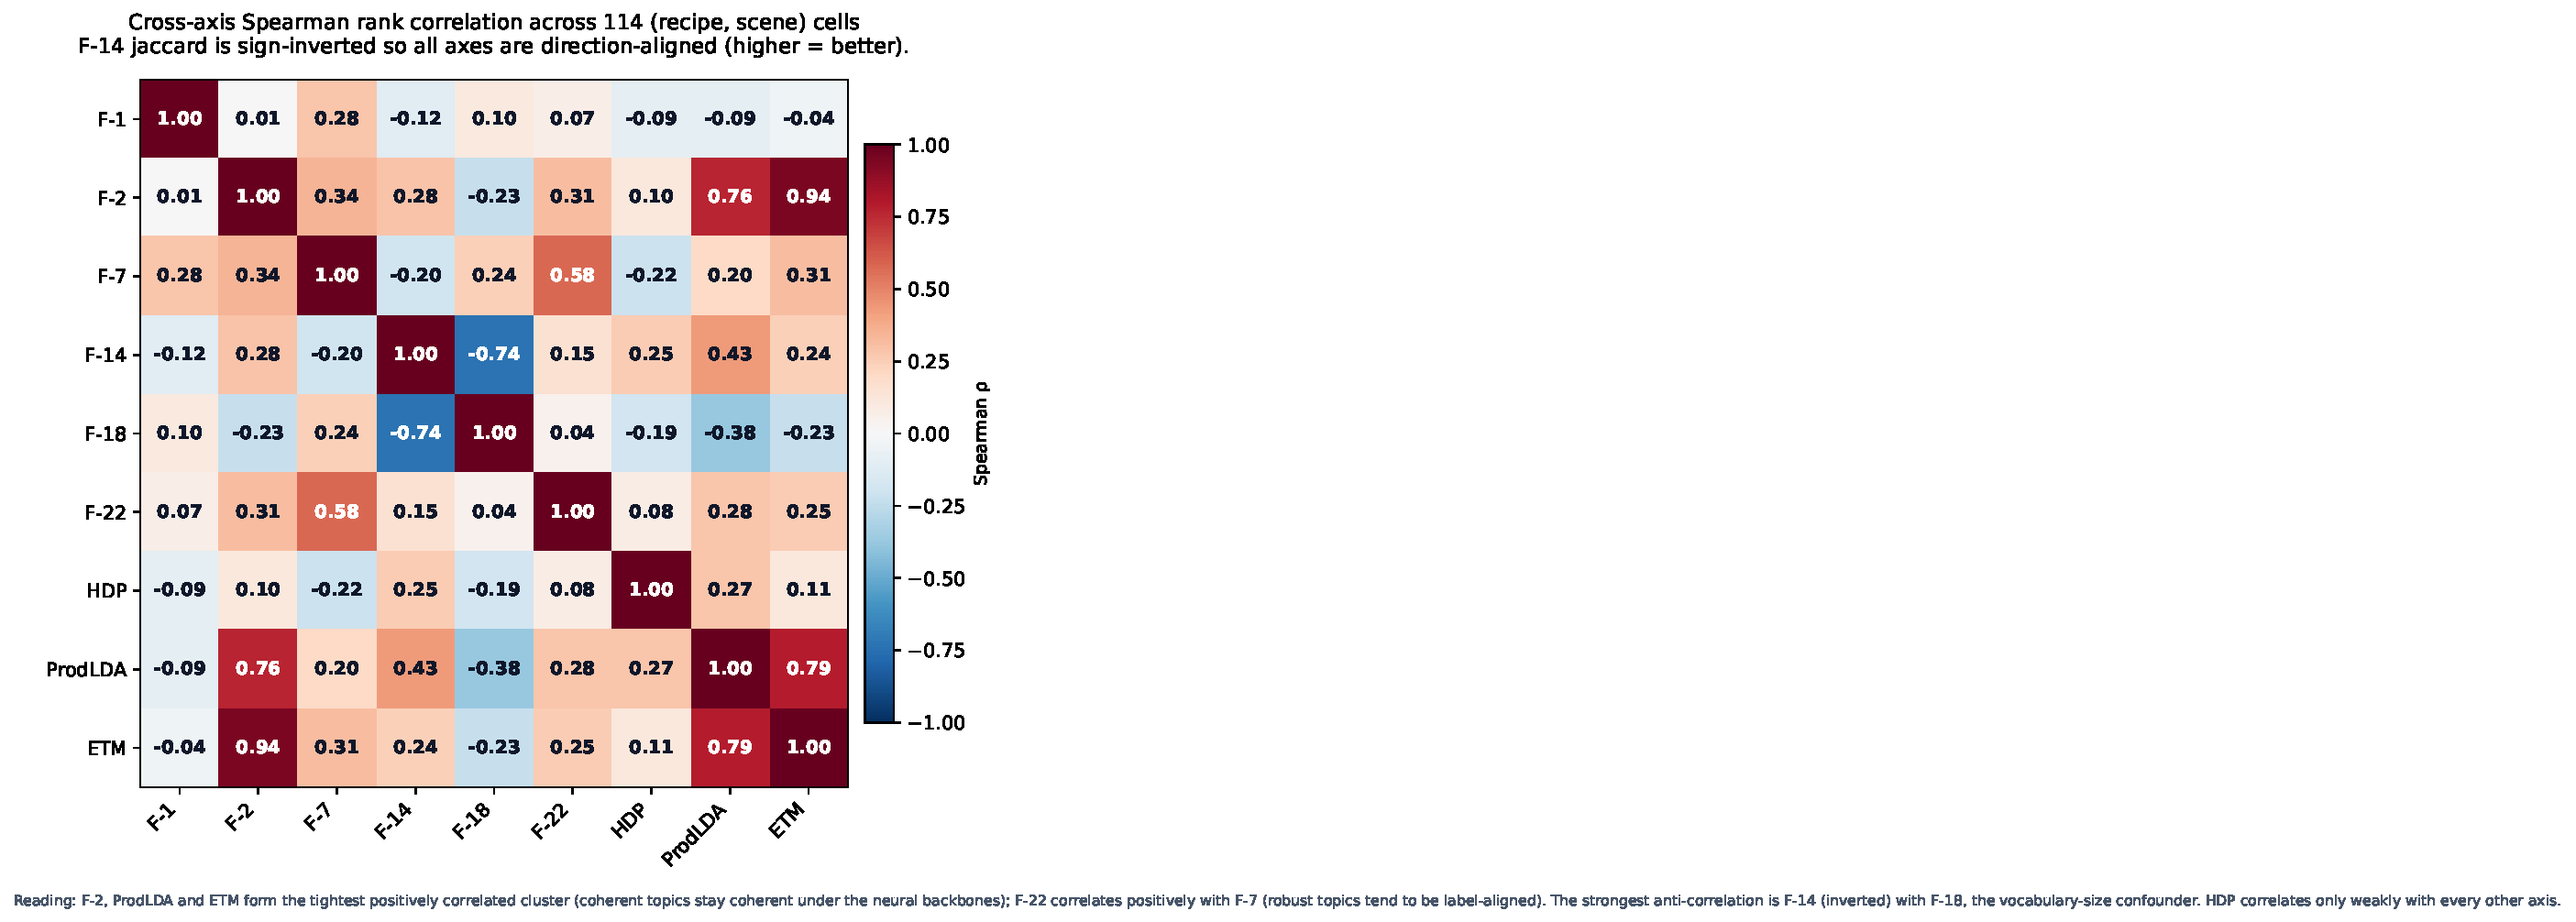
\includegraphics[width=\columnwidth,trim=18 23 826 0,clip]{p3-axis-correlation.pdf}
\caption{Spearman rank correlation across the 114 (recipe, scene)
cells; HDP, ProdLDA and ETM denote F-2 $c_v$ under that backbone.
F-14 inverted so all axes read ``higher = better''.
F-2 / ETM and F-2 / ProdLDA cluster tightly ($\rho \ge 0.76$);
F-14 anti-correlates with F-18 ($\rho = -0.74$, the vocabulary-size
confounder); F-22 / F-7 correlate at $\rho = 0.58$ (robust topics tend
to be label-aligned). The HDP column includes the V15 cells computed
on the $Q=32$ vocabulary (Fig.~\ref{fig:backbone-factorial}).}
\label{fig:corr}
\end{figure}

\paragraph{V8 stable on F-18 across $Q$} Extending F-18 to Q=16/32
on the V20 / V8 / V2 trio yields mean matched cosine across the six
labelled scenes (italic: values under the vocabulary criterion):

\begin{center}
\small
\begin{tabular}{lccc}
\toprule
Recipe & Q=8 & Q=16 & Q=32 \\
\midrule
V8 & \emph{0.957} & \emph{0.962} & \emph{0.959} \\
V2 & \emph{1.000} & 0.875 & 0.781 \\
V20 & 0.451 & 0.450 & 0.443 \\
\bottomrule
\end{tabular}
\end{center}

V8 stays between $0.957$ and $0.962$ on the F-18 mean matched cosine
across the three Q levels. Its vocabulary does not grow with $Q$ (the
same 6--12 endmember tokens at $Q = 8$, $16$ and $32$), so it meets the
vocabulary criterion at every $Q$: every matched pair has cosine at
least 0.8 whatever the fits, and these values do not measure reseed
behaviour. V20 stays near 0.45 at every $Q$, inside the range of the
per-band recipes at $Q=8$ (0.35 for V12 to 0.58 for V1). V2 falls with $Q$ ($1.000$, $0.875$
and $0.781$ at $Q = 8$, $16$ and $32$) as its vocabulary grows from 8
to 32 word types and leaves the criterion, confirming that V2's $Q=8$
value of $1.0$ is the vocabulary-size artefact flagged above.

The recommendation therefore rests on cross-backbone F-7 portability
(Table~\ref{tab:f7-4backbone} and the $Q = 16$ table above), not on
F-18: \textbf{V8 is the recipe of choice when the topic-model backbone
is uncertain}; V20 is the recipe of choice when LDA is fixed and one
can afford $Q \geq 16$ and accept the seed-sensitivity tradeoff.

% =====================================================================
\section{Four axis--recipe affinities and one hypothesis}\label{sec:affinities}
% =====================================================================

The nineteen-recipe sweep exposes four axis--recipe
affinities (\S\ref{subsec:v3-affinity}--\ref{subsec:v18-affinity}); a
fifth is a hypothesis that this study does not test
(\S\ref{subsec:v7-hypothesis}).

\subsection{V3 vs.\ F-7 topic--label coupling}
\label{subsec:v3-affinity}
In the twelve-recipe view of Table~\ref{tab:f7-full}, V3 (the joint
(band, bin) vocabulary) wins F-7 NMI on Kennedy SC (0.54), Salinas-A
(0.68) and Indian Pines (0.430 against V8's 0.428), while V12 wins on
Pavia~U (0.61) and Salinas (0.64). V3 exceeds V1 by $0.06$--$0.13$ NMI
on four of the five scenes and trails it on Salinas (0.43 vs.\ 0.47).
A likely mechanism: V3 carries
$B \times Q$ word types (1600 at $B=200, Q=8$) versus V1's $B$, and
the larger vocabulary lets a single topic concentrate on
intensity-specific band signatures that map onto land-cover classes.
On F-1 macro-F1 the recipes differ by less than 0.01
(\S\ref{sec:bayes}).

\subsection{V12 vs.\ F-2 coherence on dense regimes}
In the twelve-recipe view of Table~\ref{tab:f2-full}, V12
(Gaussian-mixture-component tokens) wins F-2 $c_v$ on Indian Pines
($c_v = 0.79$ vs.\ V1's 0.32), a scene that V20 (0.88) takes in the
nineteen-recipe sweep (Table~\ref{tab:f2-full19}), and it is
competitive on the other dense scenes. A likely reason is that the
mixture components follow the intensity distribution of the scene
instead of splitting each spectrum's range into equal bins
\eqref{eq:v12}; this study does not separate that effect from V12's
other difference from V3, the absence of per-spectrum normalisation.

\subsection{V20 vs.\ F-7 label-information-rich scenes}
\label{subsec:v20-affinity}
V20 (MI-weighted bands) wins F-7 on Indian Pines (0.44, the most
class-imbalanced scene), ties V3 on Salinas-A (0.68, the easiest scene
by F-1), and matches V12 to within $0.02$ NMI mean across the rest of
the panel. On Indian Pines its weights are broad rather than
concentrated: 169 of the 200 bands receive at least 5 of the 8
possible copies and 22 receive 3 or fewer, one of them none, so V20
differs from V3 mainly by down-weighting a minority of low-MI bands.
Its weights come from the labels that F-7 is scored against
(\S\ref{sec:results}). The recipe is parameterised by a single integer
(\texttt{MAX\_COPIES} $= 8$) and adds no per-fit cost, because the MI
estimate is computed once per scene.

\subsection{V18 vs.\ F-7 on manifold-shaped scenes}
\label{subsec:v18-affinity}
Among the unsupervised structure-aware extension recipes (V13, V17,
V18, V19), V18 (graph-Laplacian eigenvectors) has the highest F-7 NMI
on Pavia~U (0.52) and Salinas (0.50, Table~\ref{tab:f7-extension}), and
it places third on F-7 mean among the extension recipes (0.43 NMI).
Against all nineteen recipes it leads neither scene. The intuition: scenes whose labelled classes
correspond to connected regions in the pixel-similarity graph (urban
land-cover types in Pavia, agricultural fields in Salinas) yield
informative Laplacian eigenvectors whose low frequencies group those
regions. Bin-tokens over those eigenvectors then carry segmentation
semantics that LDA can fit topics around. The result is a recipe that
explicitly exposes the manifold structure to the topic model.

\subsection{V7 vs.\ F-9 HIDSAG cross-preprocessing
(hypothesis)}
\label{subsec:v7-hypothesis}
This fifth affinity is a hypothesis that the present study does not
test: F-9 is not swept (\S\ref{sec:limitations}). V7 is the most
chemistry-faithful recipe (centroid, depth, area triplets), and we
expect it to dominate on the HIDSAG mineralogical subsets, where
USGS-library matching is the gold standard.

% =====================================================================
\section{Recommendation: V1 as canonical default, not universal best}
\label{sec:recommendation}
% =====================================================================

The sweep supports a sharper statement about V1's
role: V1 should remain canonical as a \emph{reproducibility default}
(deterministic, dense, well-understood, and the band--frequency
representation of the geometallurgical study~\cite{santibanezleal2022procemin}
that V1--V3 generalise) but should not be claimed as a universal best. P1's
framework results, computed on V1, are stable benchmarks; a future
study comparing V1 against, say, V3 or V12 on F-7 would need to refit.
The proposed convention is to report every framework result against
V1 alongside the per-axis best recipe.

% =====================================================================
\section{Limitations and future work}\label{sec:limitations}
% =====================================================================

\begin{itemize}
  \item \textbf{V11 reproducibility}: the implementation does not pin
    a random seed for the nanopq codebook fit, so the V11 results
    reported here come from a single unseeded codebook fit and may
    change when the seed is pinned and the cells are recomputed.
  \item \textbf{$c_{\mathrm{NPMI}}$ on dense recipes}: V1 (and any other recipe
    with mean doc length close to $|\mathcal{V}|$) produces a degenerate
    pixel-as-document NPMI because nearly every word fires in every document.
    A sliding-window estimator would yield comparable numbers; we
    leave that to a follow-up.
  \item \textbf{F-3 / F-4 / F-5 / F-8 / F-9 / F-10 / F-11 / F-12
    not swept}: the sweep reports F-1, F-2 and F-7, together with the
    extension axes of \S\ref{sec:extensions}. The remaining framework
    axes are left to future work, either as an extension of this
    study or as a separate one.
  \item \textbf{V16 foundation-model embeddings not built}: V16 is
    reserved for a foundation-model wordification (HyperSIGMA,
    HyperspectralMAE, or SatMAE) that embeds each pixel into a learnt
    latent space and quantises that into LDA tokens. Building V16
    requires GPU inference at scene scale, which exceeds the
    single-node computational resources used in this study. We expect
    V16 to set the upper bound for F-7 NMI on the panel; its slot in
    the recipe index is reserved for that follow-up.
  \item \textbf{Full backbone factorial at $Q = 8$ only}: at $Q = 8$ the
    factorial covers all nineteen recipes on the six labelled scenes
    under the four backbones, for F-2 (456 cells,
    Fig.~\ref{fig:backbone-factorial}) and F-7 (456 cells,
    Table~\ref{tab:f7-4backbone}). At $Q = 16$ the HDP, ProdLDA and
    ETM backbones cover only V2, V8 and V20, and $Q = 32$ is run under
    LDA only.
\end{itemize}

% =====================================================================
\section{Conclusion}\label{sec:conclusion}
% =====================================================================

A nineteen-recipe sweep of the wordification step, evaluated on the
F-1, F-2 and F-7 axes of the twelve-axis framework of the companion
paper and on five extension axes, shows that
\emph{no single recipe is universally best}. On classification (F-1,
\eqref{eq:f1}) the recipes differ consistently but by less than 0.01
macro-F1 (V12 leads, \S\ref{sec:bayes}); the discriminating axes are coherence (F-2,
\eqref{eq:f2}) and topic--label coupling (F-7, \eqref{eq:f7}), where
the spread between the best and worst recipe mean reaches $0.65$ and
$0.43$ respectively (Tables \ref{tab:f2-full} and \ref{tab:f7-full}).
The same three
recipes, V12 \eqref{eq:v12} (Gaussian-mixture tokens), V3
\eqref{eq:v3} (joint band--bin vocabulary) and V20 \eqref{eq:v20}
(mutual-information-weighted bands), have the three highest six-scene
means on both F-2 and F-7, and on F-7 they lie within $0.014$ NMI of
each other, a flat design-space ceiling rather than a sharp peak.
V20, the simplest label-aware reweighting of V3 \eqref{eq:v3}, wins
F-2 and F-7 together on Indian Pines (its weights use the labels that
F-7 is scored against) and has the highest F-22 of the sweep
(\eqref{eq:f22}, $L_1 = 26.3$, a count that grows with its longer
documents); its F-7 lead grows with quantiser resolution, reaching the
highest absolute F-7 at $Q = 32$. The
cross-backbone factorial identifies V8 \eqref{eq:v8} (NFINDR
endmember-fraction) as the most backbone-portable recipe; its F-18
values (\eqref{eq:f18}, $\ge 0.95$) are bounded below by 0.8 through
its 6--12-token endmember vocabulary and do not measure reseed
reliability. The practical
recommendation is twofold: retain V1 as a \emph{reproducibility
default} rather than a universal best, and pick the recipe to the
axis: V20 when LDA is fixed and finer quantisation is affordable,
V8 when the backbone is uncertain.
Closing the remaining framework axes (F-3--F-12) over the full
nineteen-recipe family, and building the deferred foundation-model
wordification V16, are the natural next steps.

% =====================================================================
\section*{Data availability}
% =====================================================================

{\raggedright
Per-cell results (one JSON record per scene, recipe and quantisation
level) are archived in the code repository
\url{https://github.com/fsantibanezleal/CAOS_LDA_HSI} under
\path{data/derived/v_sweep/}: \path{f1_per_fold/} (with the unpaired
bootstrap summary in \path{f1_bootstrap_posterior.json}; the paired
comparison of \S\ref{sec:bayes} and Table~\ref{tab:f1-full19} are
computed from these records by \path{scripts/f1_paired_bootstrap.py}
of the manuscript repository),
\path{f2_coherence/}, \path{f7_topic_to_label/}, \path{f13_shap/},
\path{f14_repetitiveness/}, \path{f17_cross_scene/},
\path{f18_reliability/} and \path{f22_counterfactual/} for the LDA
axes; \path{hdp_backbone/},
\path{prodlda_backbone/} and \path{etm_backbone/} (F-2) and
\path{backbones_f7/} (F-7) for the backbone factorial. The same folder
holds runs on the five HIDSAG subsets~\cite{hidsag2023}
(\path{hidsag/}: F-2, F-14 and topic-to-owner mutual information for
fifteen recipes), which this paper does not analyse.\par}

% =====================================================================
\appendices
\section{Full nineteen-recipe F-1, F-2 and F-7 matrices}
\label{app:full-matrix}
% =====================================================================

Tables~\ref{tab:f1-full19}, \ref{tab:f2-full19} and~\ref{tab:f7-full19}
report F-1 macro-F1, F-2 $c_v$ and F-7 NMI for all nineteen recipes on
the six labelled scenes.

\begin{table*}[ht]
\caption{F-1 mean macro-F1 (topic\_routed\_soft, 5 folds) across the
full V1--V15, V17--V20 sweep on the labelled-scene panel. Bold = best
per scene at full precision, exact ties included (V8 leads V3 on
Botswana by 0.0007).}
\label{tab:f1-full19}
\centering
\scriptsize
\setlength{\tabcolsep}{2.2pt}
\begin{tabular}{l*{19}{c}}
\toprule
Scene & V1 & V2 & V3 & V4 & V5 & V6 & V7 & V8 & V9 & V10 & V11 & V12 & V13 & V14 & V15 & V17 & V18 & V19 & V20 \\
\midrule
Botswana     & 0.963 & 0.965 & 0.966 & 0.964 & 0.963 & 0.959 & 0.963 & \textbf{0.966} & 0.962 & 0.965 & 0.963 & 0.965 & 0.964 & 0.964 & 0.962 & 0.963 & 0.965 & 0.965 & 0.964 \\
Indian Pines & 0.842 & \textbf{0.861} & 0.852 & 0.844 & 0.841 & 0.839 & 0.840 & 0.850 & 0.845 & 0.842 & 0.845 & 0.853 & 0.839 & 0.847 & 0.844 & 0.843 & 0.837 & 0.840 & 0.858 \\
Kennedy SC   & 0.923 & 0.921 & 0.923 & 0.919 & 0.920 & 0.919 & 0.916 & 0.920 & 0.919 & 0.916 & 0.915 & \textbf{0.930} & 0.919 & 0.917 & 0.919 & 0.920 & 0.919 & 0.918 & 0.921 \\
Pavia U      & 0.815 & 0.804 & 0.805 & 0.818 & 0.815 & 0.815 & 0.821 & 0.814 & 0.813 & 0.808 & 0.828 & \textbf{0.834} & 0.805 & 0.811 & 0.814 & 0.803 & 0.810 & 0.805 & 0.811 \\
Salinas-A    & \textbf{0.997} & 0.996 & 0.996 & 0.996 & 0.996 & \textbf{0.997} & 0.996 & 0.995 & 0.996 & 0.996 & 0.996 & 0.996 & \textbf{0.997} & \textbf{0.997} & 0.996 & 0.996 & \textbf{0.997} & 0.996 & \textbf{0.997} \\
Salinas      & 0.951 & \textbf{0.956} & 0.950 & 0.950 & 0.952 & 0.951 & 0.948 & 0.952 & 0.951 & 0.952 & 0.950 & 0.952 & 0.952 & 0.951 & 0.954 & 0.950 & 0.951 & 0.949 & 0.950 \\
\midrule
mean         & 0.915 & 0.917 & 0.915 & 0.915 & 0.914 & 0.913 & 0.914 & 0.916 & 0.914 & 0.913 & 0.916 & \textbf{0.922} & 0.912 & 0.915 & 0.915 & 0.913 & 0.913 & 0.912 & 0.917 \\
\bottomrule
\end{tabular}
\end{table*}

\begin{table*}[ht]
\caption{F-2 $c_v$ across the full V1--V15, V17--V20 sweep on the
labelled-scene panel. Bold = best per scene across all 19 recipes.}
\label{tab:f2-full19}
\centering
\scriptsize
\setlength{\tabcolsep}{3pt}
\begin{tabular}{l*{19}{c}}
\toprule
Scene & V1 & V2 & V3 & V4 & V5 & V6 & V7 & V8 & V9 & V10 & V11 & V12 & V13 & V14 & V15 & V17 & V18 & V19 & V20 \\
\midrule
Indian Pines & 0.32 & 0.35 & 0.70 & 0.32 & 0.32 & 0.32 & 0.27 & 0.30 & 0.71 & 0.27 & 0.24 & 0.79 & 0.29 & 0.46 & 0.29 & 0.34 & 0.58 & 0.37 & \textbf{0.88} \\
Salinas      & 0.36 & 0.35 & 0.65 & 0.32 & 0.32 & 0.32 & 0.20 & 0.21 & 0.72 & 0.29 & 0.22 & \textbf{0.84} & 0.29 & 0.53 & 0.36 & 0.59 & 0.51 & 0.32 & 0.80 \\
Salinas-A    & \textbf{0.96} & 0.35 & 0.92 & 0.32 & 0.32 & 0.81 & 0.32 & 0.38 & 0.71 & 0.23 & 0.21 & 0.88 & 0.22 & 0.72 & 0.39 & 0.45 & 0.52 & 0.38 & 0.74 \\
Pavia U      & 0.91 & 0.43 & 0.96 & 0.59 & 0.40 & 0.58 & 0.27 & 0.21 & 0.70 & 0.32 & 0.22 & \textbf{1.00} & 0.28 & 0.76 & 0.25 & 0.40 & 0.66 & 0.39 & 0.95 \\
Kennedy SC   & \textbf{0.97} & 0.76 & 0.93 & 0.81 & 0.93 & 0.79 & 0.37 & 0.52 & 0.72 & 0.53 & 0.25 & 0.89 & 0.26 & 0.76 & 0.50 & 0.42 & 0.63 & 0.41 & 0.88 \\
Botswana     & 0.35 & 0.35 & \textbf{0.90} & 0.32 & 0.32 & 0.34 & 0.33 & 0.29 & 0.70 & 0.33 & 0.26 & 0.85 & 0.17 & 0.52 & 0.39 & 0.34 & 0.50 & 0.38 & 0.85 \\
\bottomrule
\end{tabular}
\end{table*}

\begin{table*}[ht]
\caption{F-7 NMI across the full V1--V15, V17--V20 sweep on the
labelled-scene panel. Bold = best per scene across all 19 recipes.}
\label{tab:f7-full19}
\centering
\scriptsize
\setlength{\tabcolsep}{3pt}
\begin{tabular}{l*{19}{c}}
\toprule
Scene & V1 & V2 & V3 & V4 & V5 & V6 & V7 & V8 & V9 & V10 & V11 & V12 & V13 & V14 & V15 & V17 & V18 & V19 & V20 \\
\midrule
Indian Pines & 0.34 & 0.35 & 0.43 & 0.25 & 0.20 & 0.25 & 0.16 & 0.43 & 0.10 & 0.08 & 0.25 & 0.42 & 0.29 & 0.31 & 0.26 & 0.18 & 0.27 & 0.21 & \textbf{0.44} \\
Salinas      & 0.47 & 0.54 & 0.43 & 0.39 & 0.44 & 0.32 & 0.28 & 0.56 & 0.14 & 0.20 & 0.33 & \textbf{0.64} & 0.35 & 0.51 & 0.28 & 0.17 & 0.50 & 0.35 & 0.47 \\
Salinas-A    & 0.62 & 0.64 & \textbf{0.68} & 0.37 & 0.56 & 0.33 & 0.16 & 0.52 & 0.20 & 0.28 & 0.42 & 0.55 & 0.49 & 0.55 & 0.51 & 0.34 & 0.52 & 0.33 & 0.68 \\
Pavia U      & 0.47 & 0.38 & 0.55 & 0.38 & 0.14 & 0.43 & 0.23 & 0.54 & 0.02 & 0.00 & 0.21 & \textbf{0.61} & 0.22 & 0.49 & 0.28 & 0.21 & 0.52 & 0.36 & 0.54 \\
Kennedy SC   & 0.41 & 0.40 & \textbf{0.54} & 0.32 & 0.25 & 0.34 & 0.20 & 0.17 & 0.11 & 0.17 & 0.22 & 0.51 & 0.31 & 0.43 & 0.29 & 0.21 & 0.28 & 0.25 & 0.52 \\
Botswana     & 0.42 & 0.40 & 0.52 & 0.35 & 0.20 & 0.24 & 0.17 & \textbf{0.56} & 0.13 & 0.17 & 0.32 & 0.46 & 0.21 & 0.44 & 0.25 & 0.19 & 0.47 & 0.21 & 0.47 \\
\midrule
mean         & 0.45 & 0.45 & 0.52 & 0.35 & 0.30 & 0.32 & 0.20 & 0.46 & 0.12 & 0.15 & 0.29 & \textbf{0.53} & 0.31 & 0.46 & 0.31 & 0.22 & 0.43 & 0.29 & 0.52 \\
\bottomrule
\end{tabular}
\end{table*}

% =====================================================================
\bibliographystyle{IEEEtran}
\bibliography{../../bibliography/refs,companion}

\end{document}
